$\beta = 1$, $H = 1$ and $t_f = 10\sec$.
Now we simulate our system for $\alpha = 1, 5, 10$ and plot $K(t)$ matrix, $u(t)$ and states of system.
\begin{itemize}
	%%%%%%%%% alpha = 1 %%%%%%%%%
	\item $\alpha = 1$
	%%%%%%% K(t) %%%%%%%
		\begin{figure}[H]
		\caption{$K(t)$ in $\alpha = 1$}
		\centering
		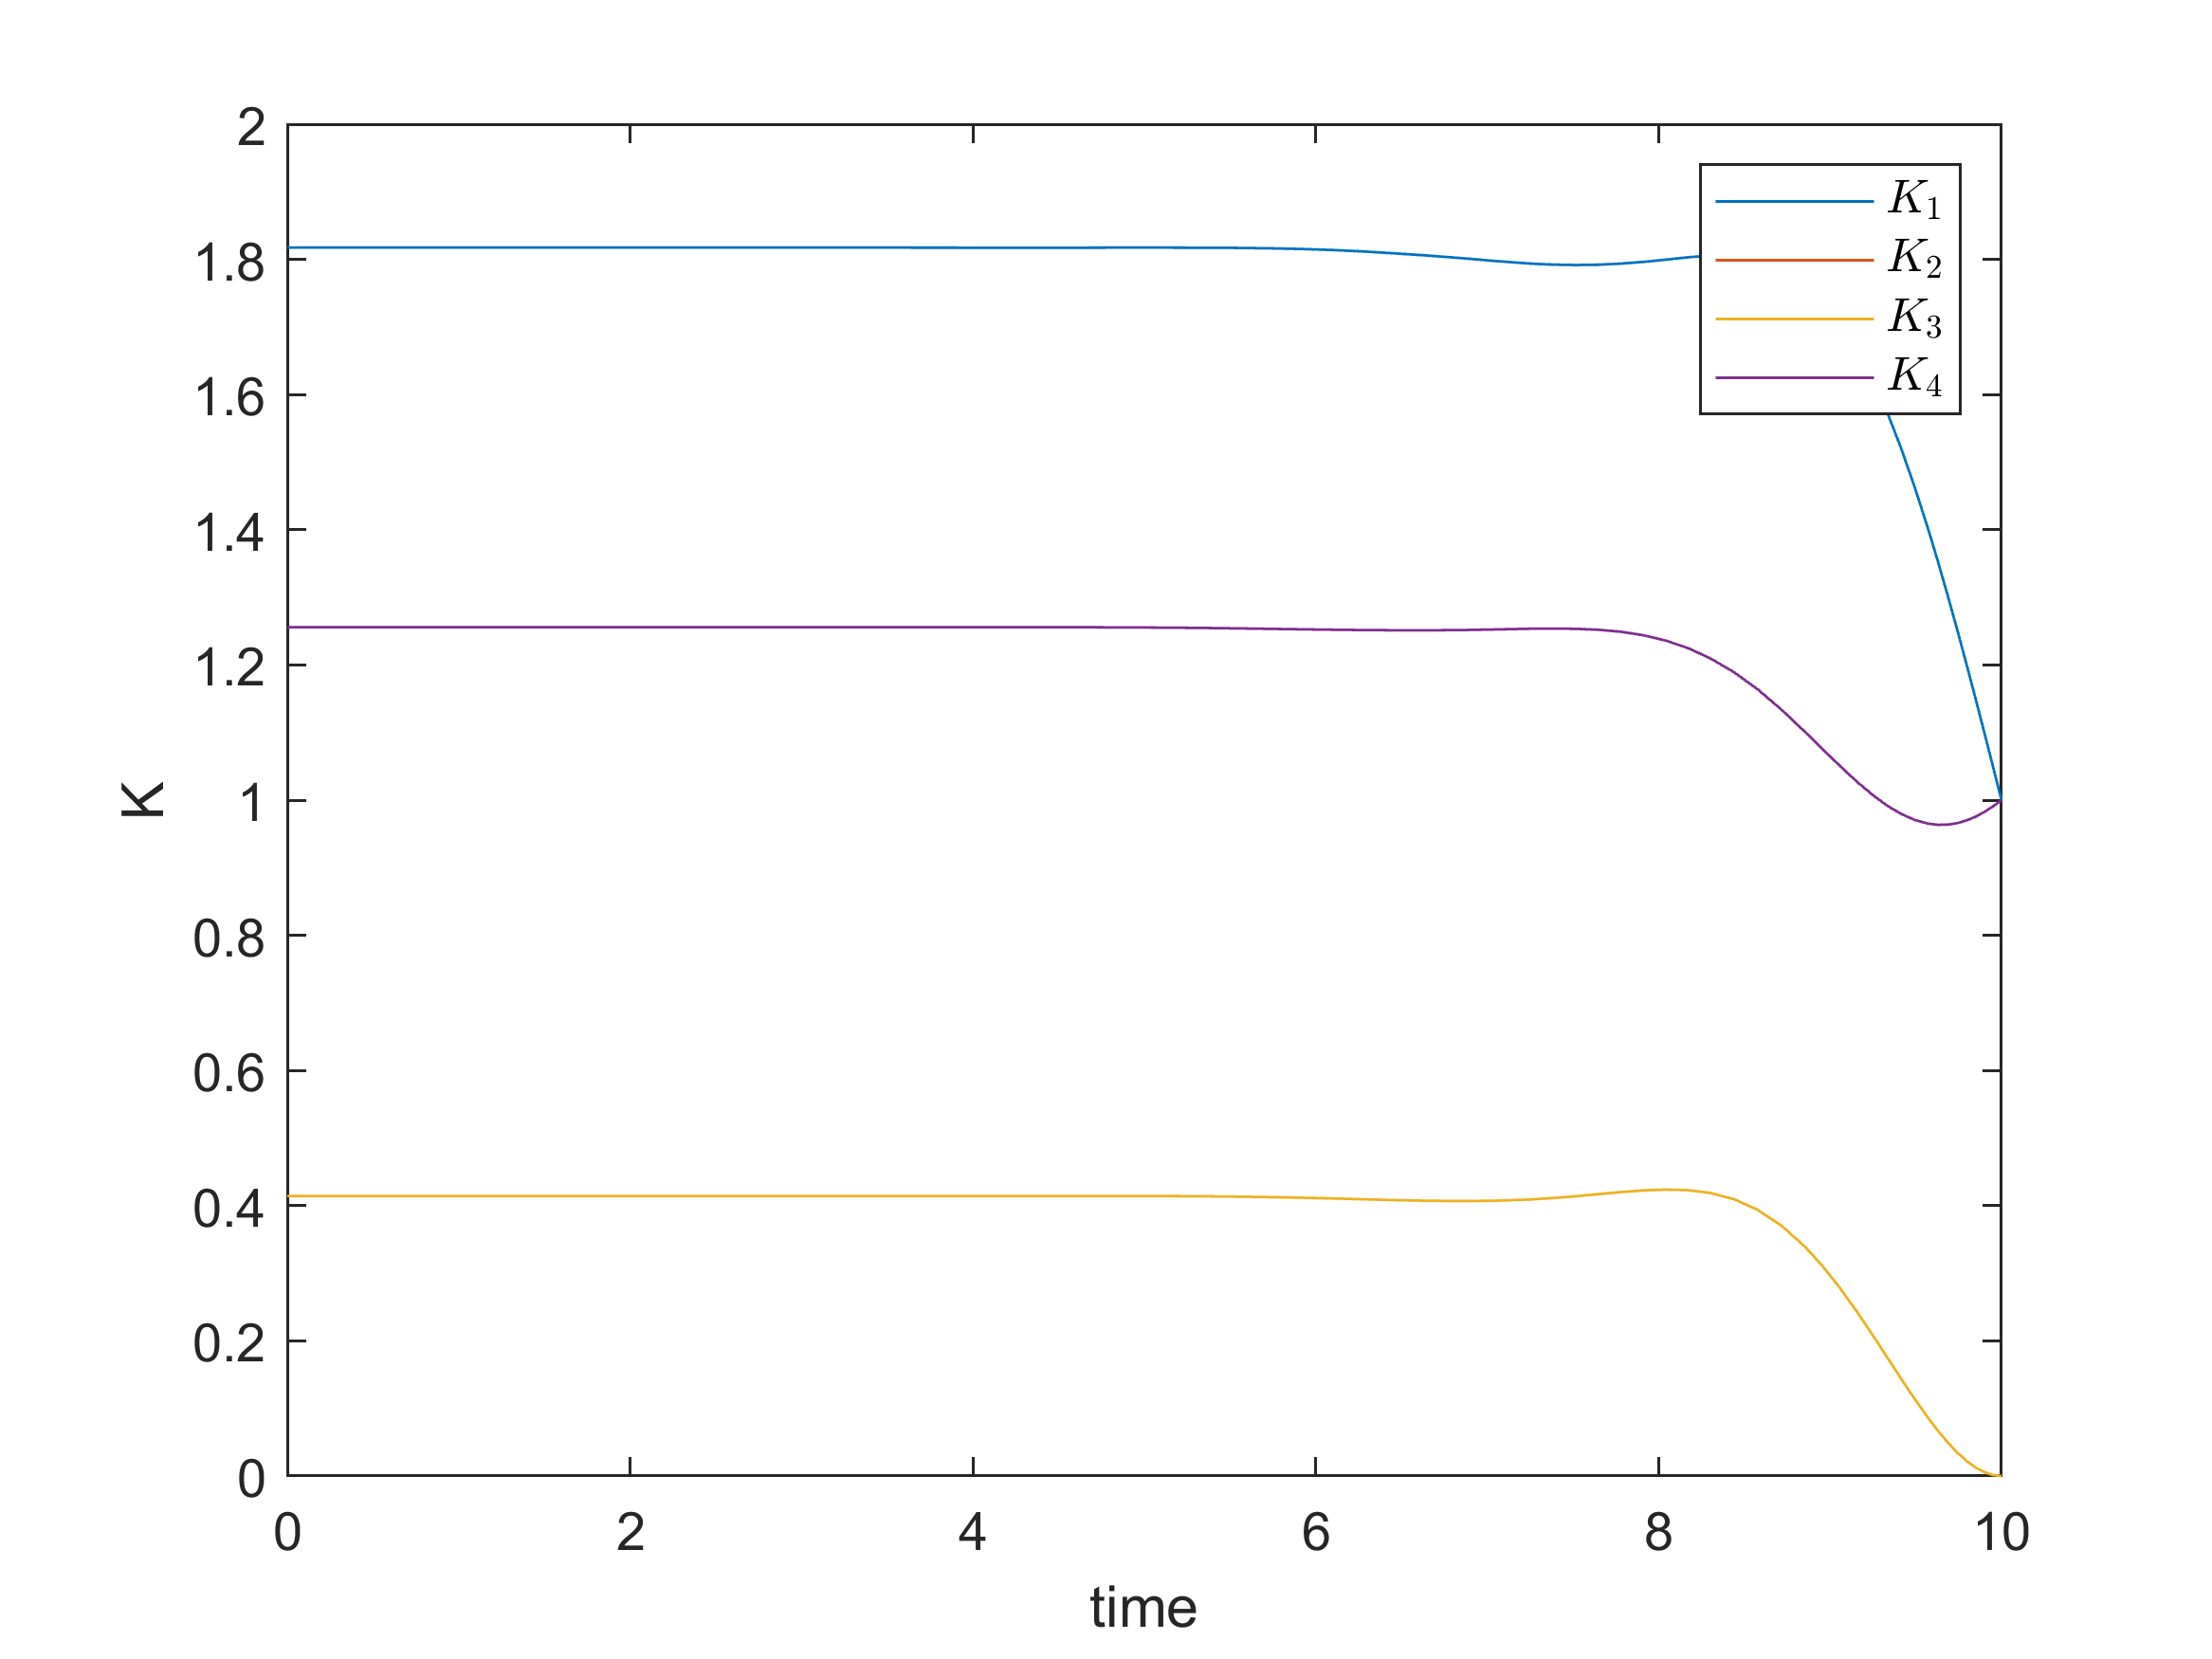
\includegraphics[width=12cm]{../Code/Q3/figures/Kalpha1.png}
	\end{figure}
%%%%%%% u(t) %%%%%%%
		\begin{figure}[H]
	\caption{$u(t)$ in $\alpha = 1$}
	\centering
	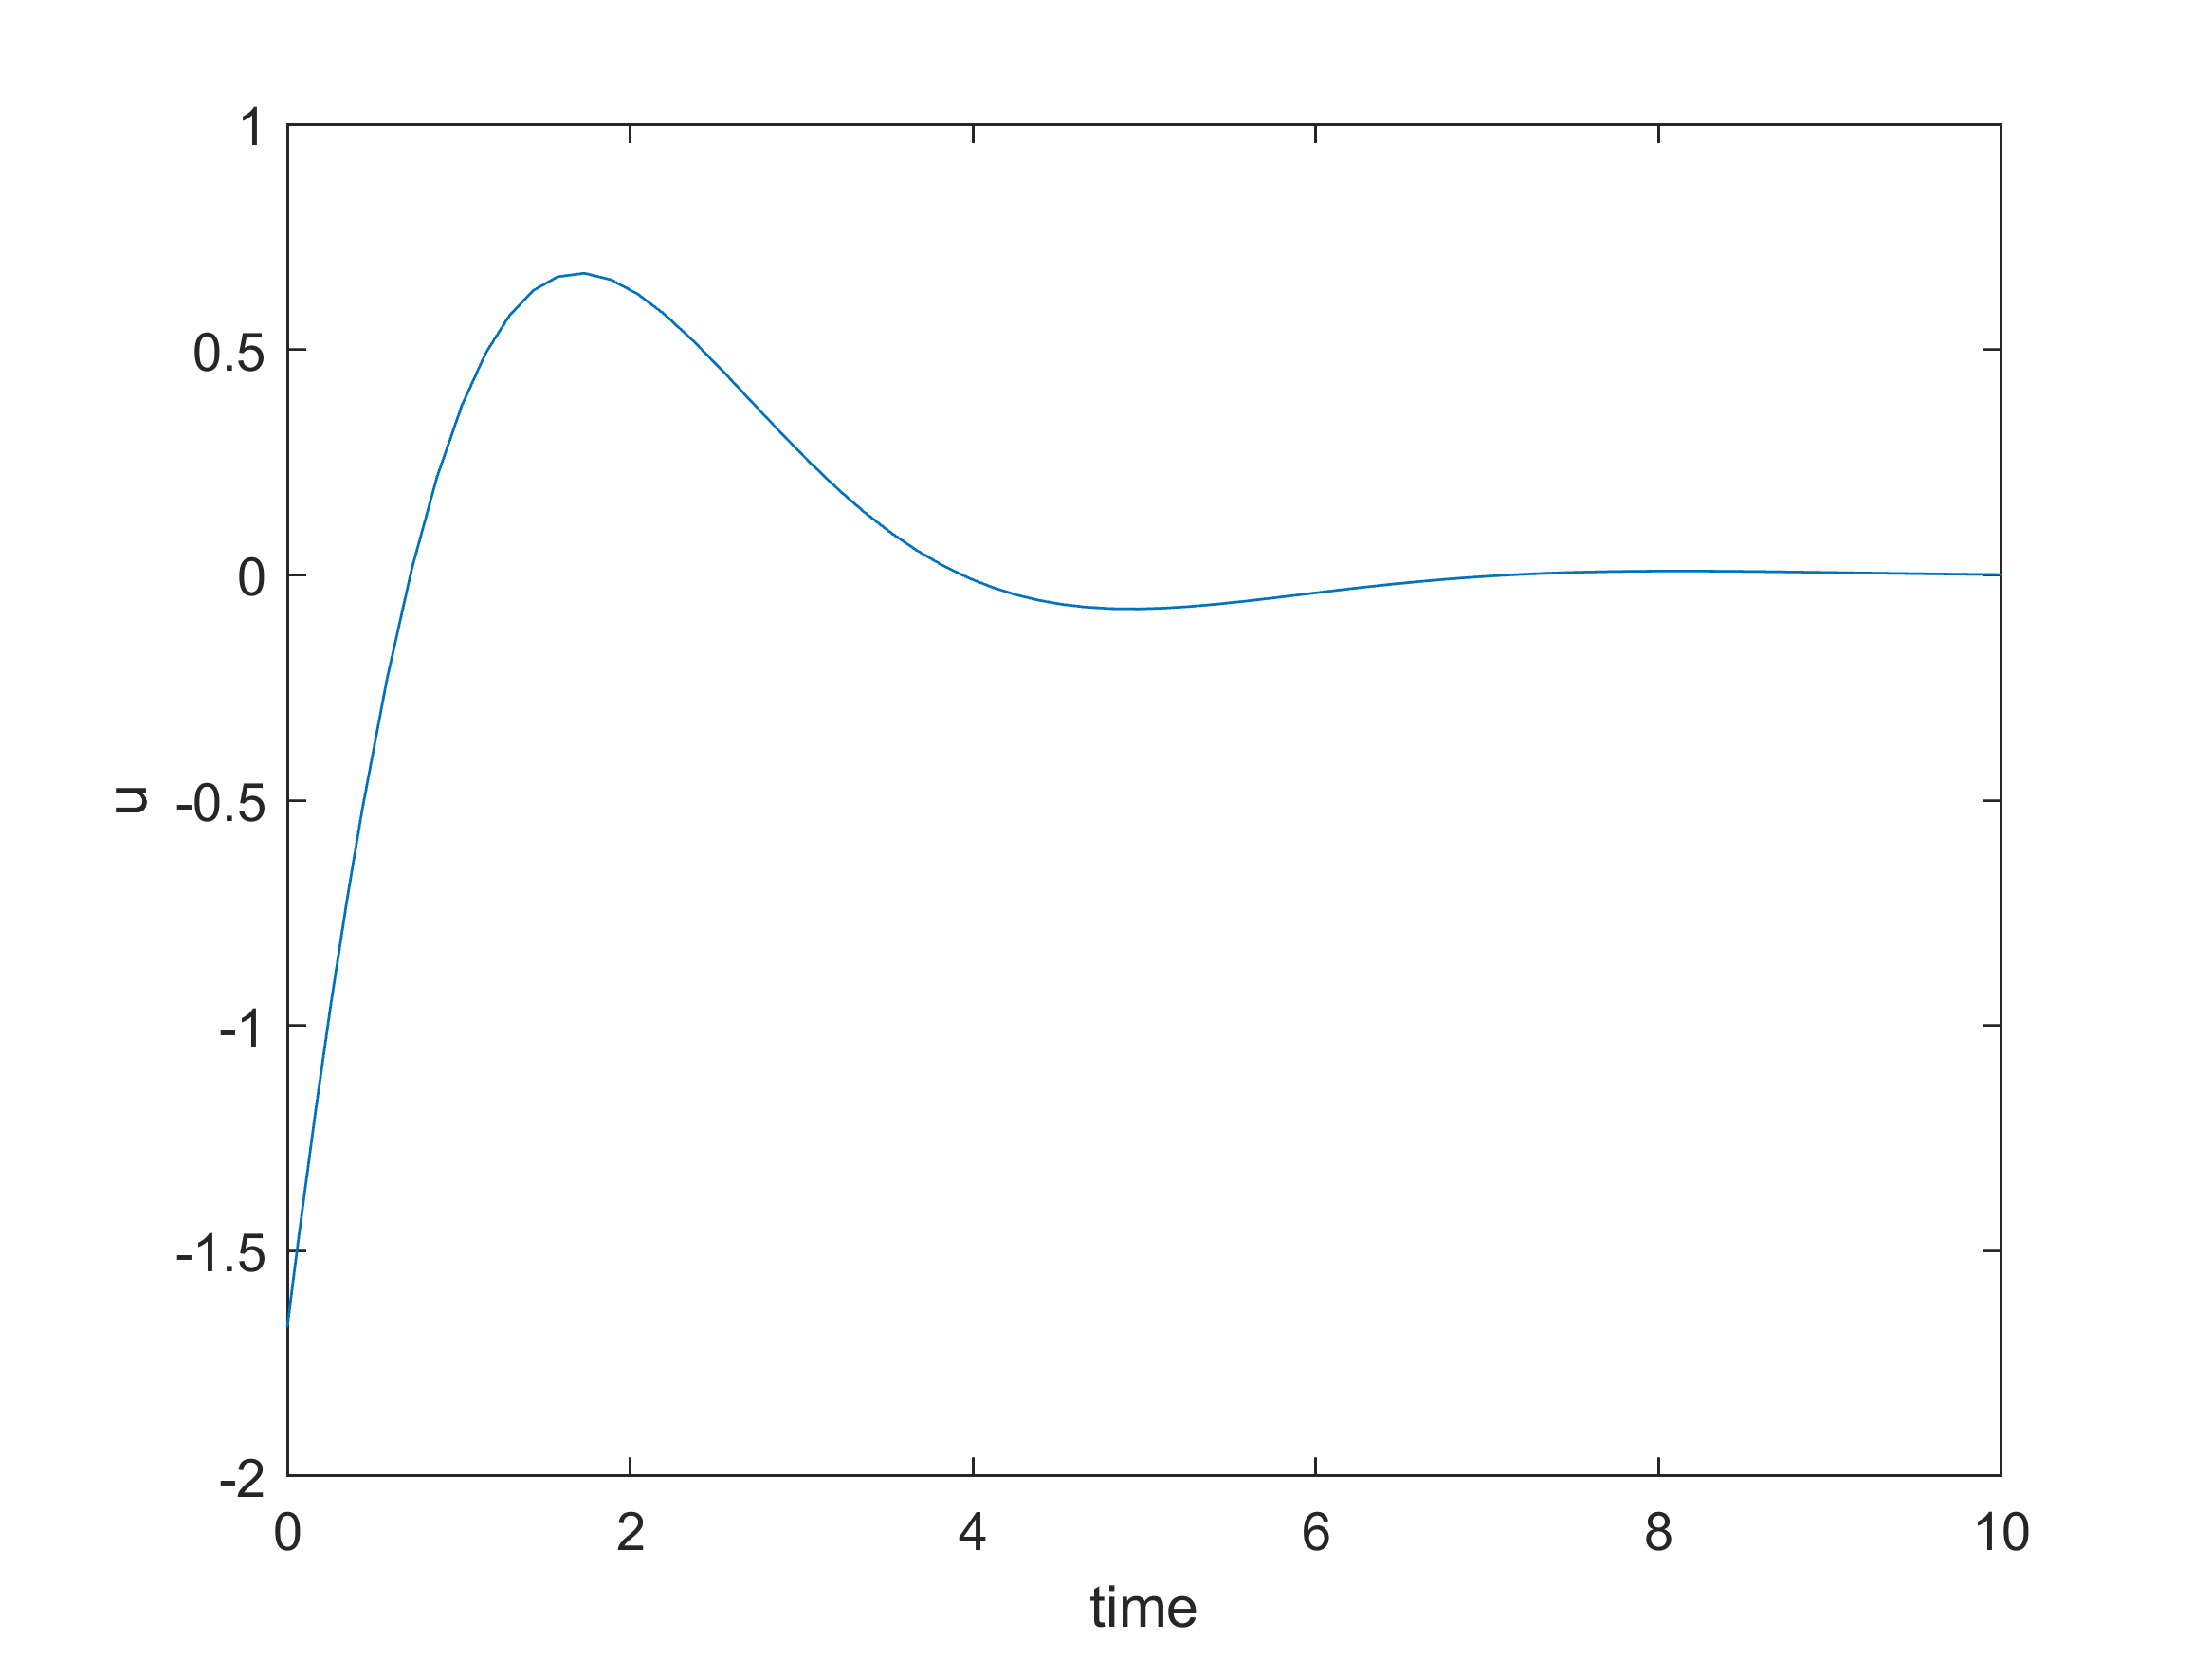
\includegraphics[width=12cm]{../Code/Q3/figures/ualpha1.png}
\end{figure}
%%%%%%% x(t) %%%%%%%
		\begin{figure}[H]
	\caption{System States $\vec x(t)$ in $\alpha = 1$}
	\centering
	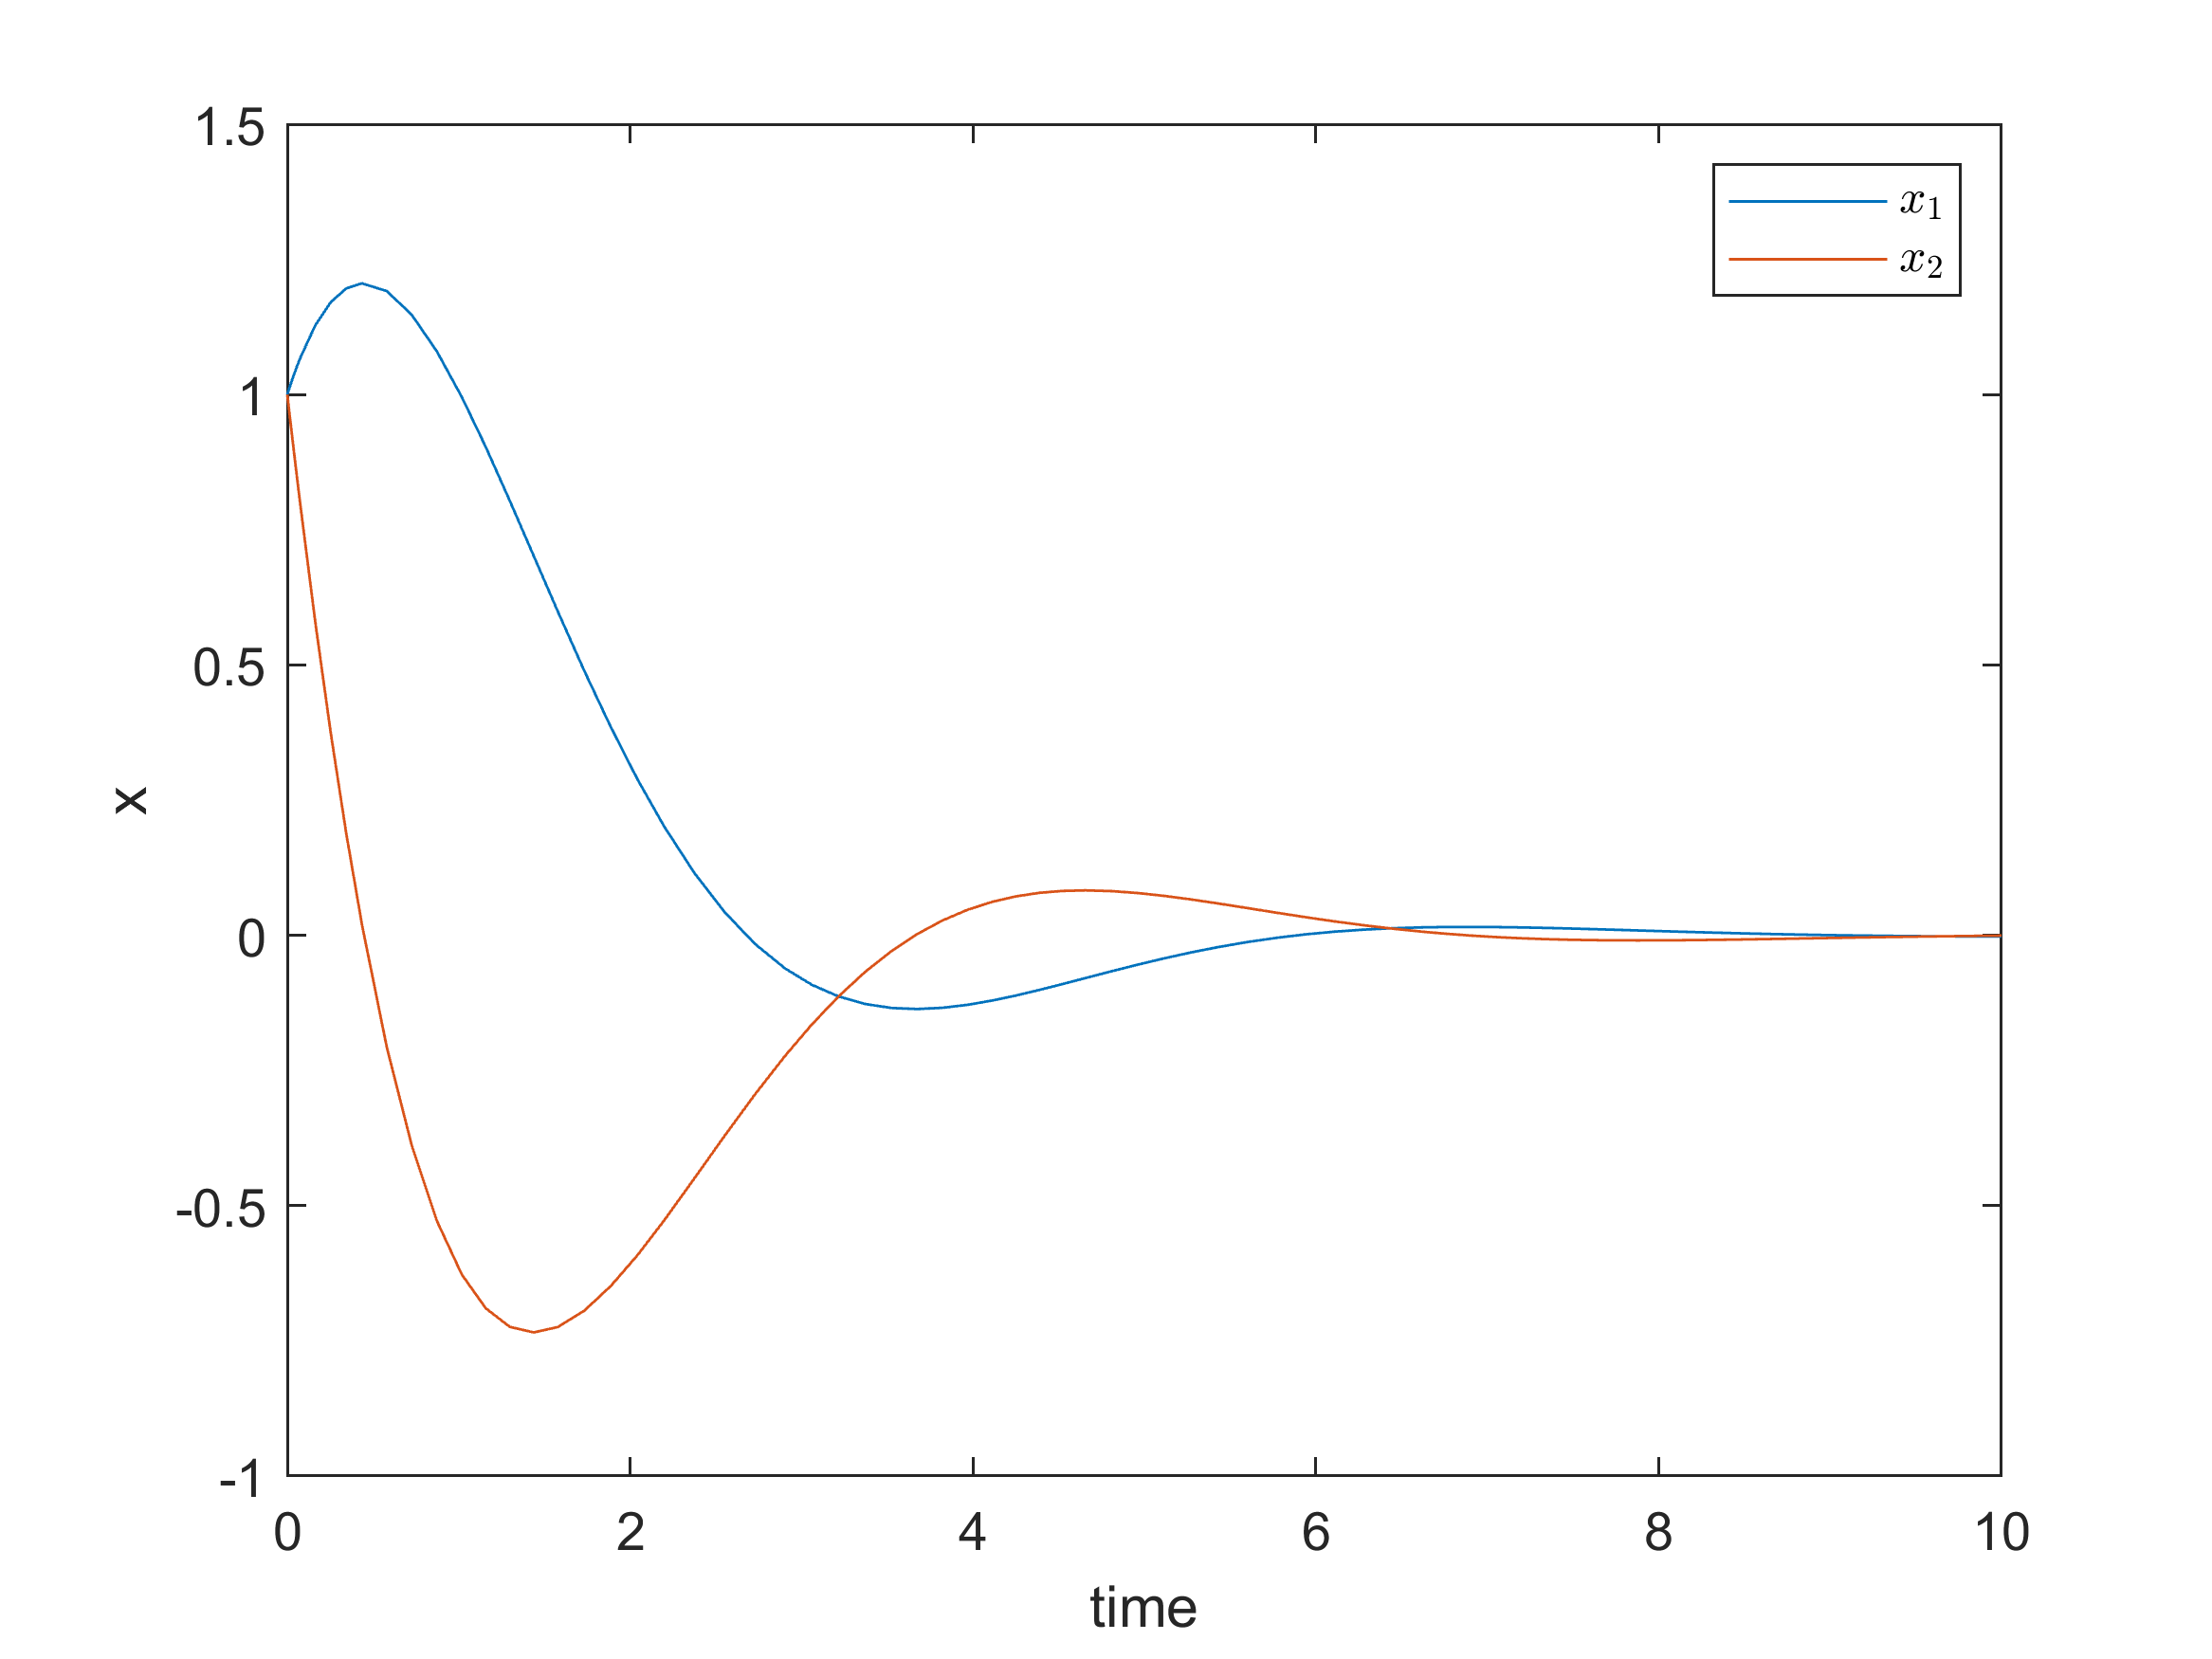
\includegraphics[width=12cm]{../Code/Q3/figures/xalpha1.png}
\end{figure}
	%%%%%%%%% alpha = 5 %%%%%%%%%
\item $\alpha = 5$
%%%%%%% K(t) %%%%%%%
\begin{figure}[H]
	\caption{$K(t)$ in $\alpha = 5$}
	\centering
	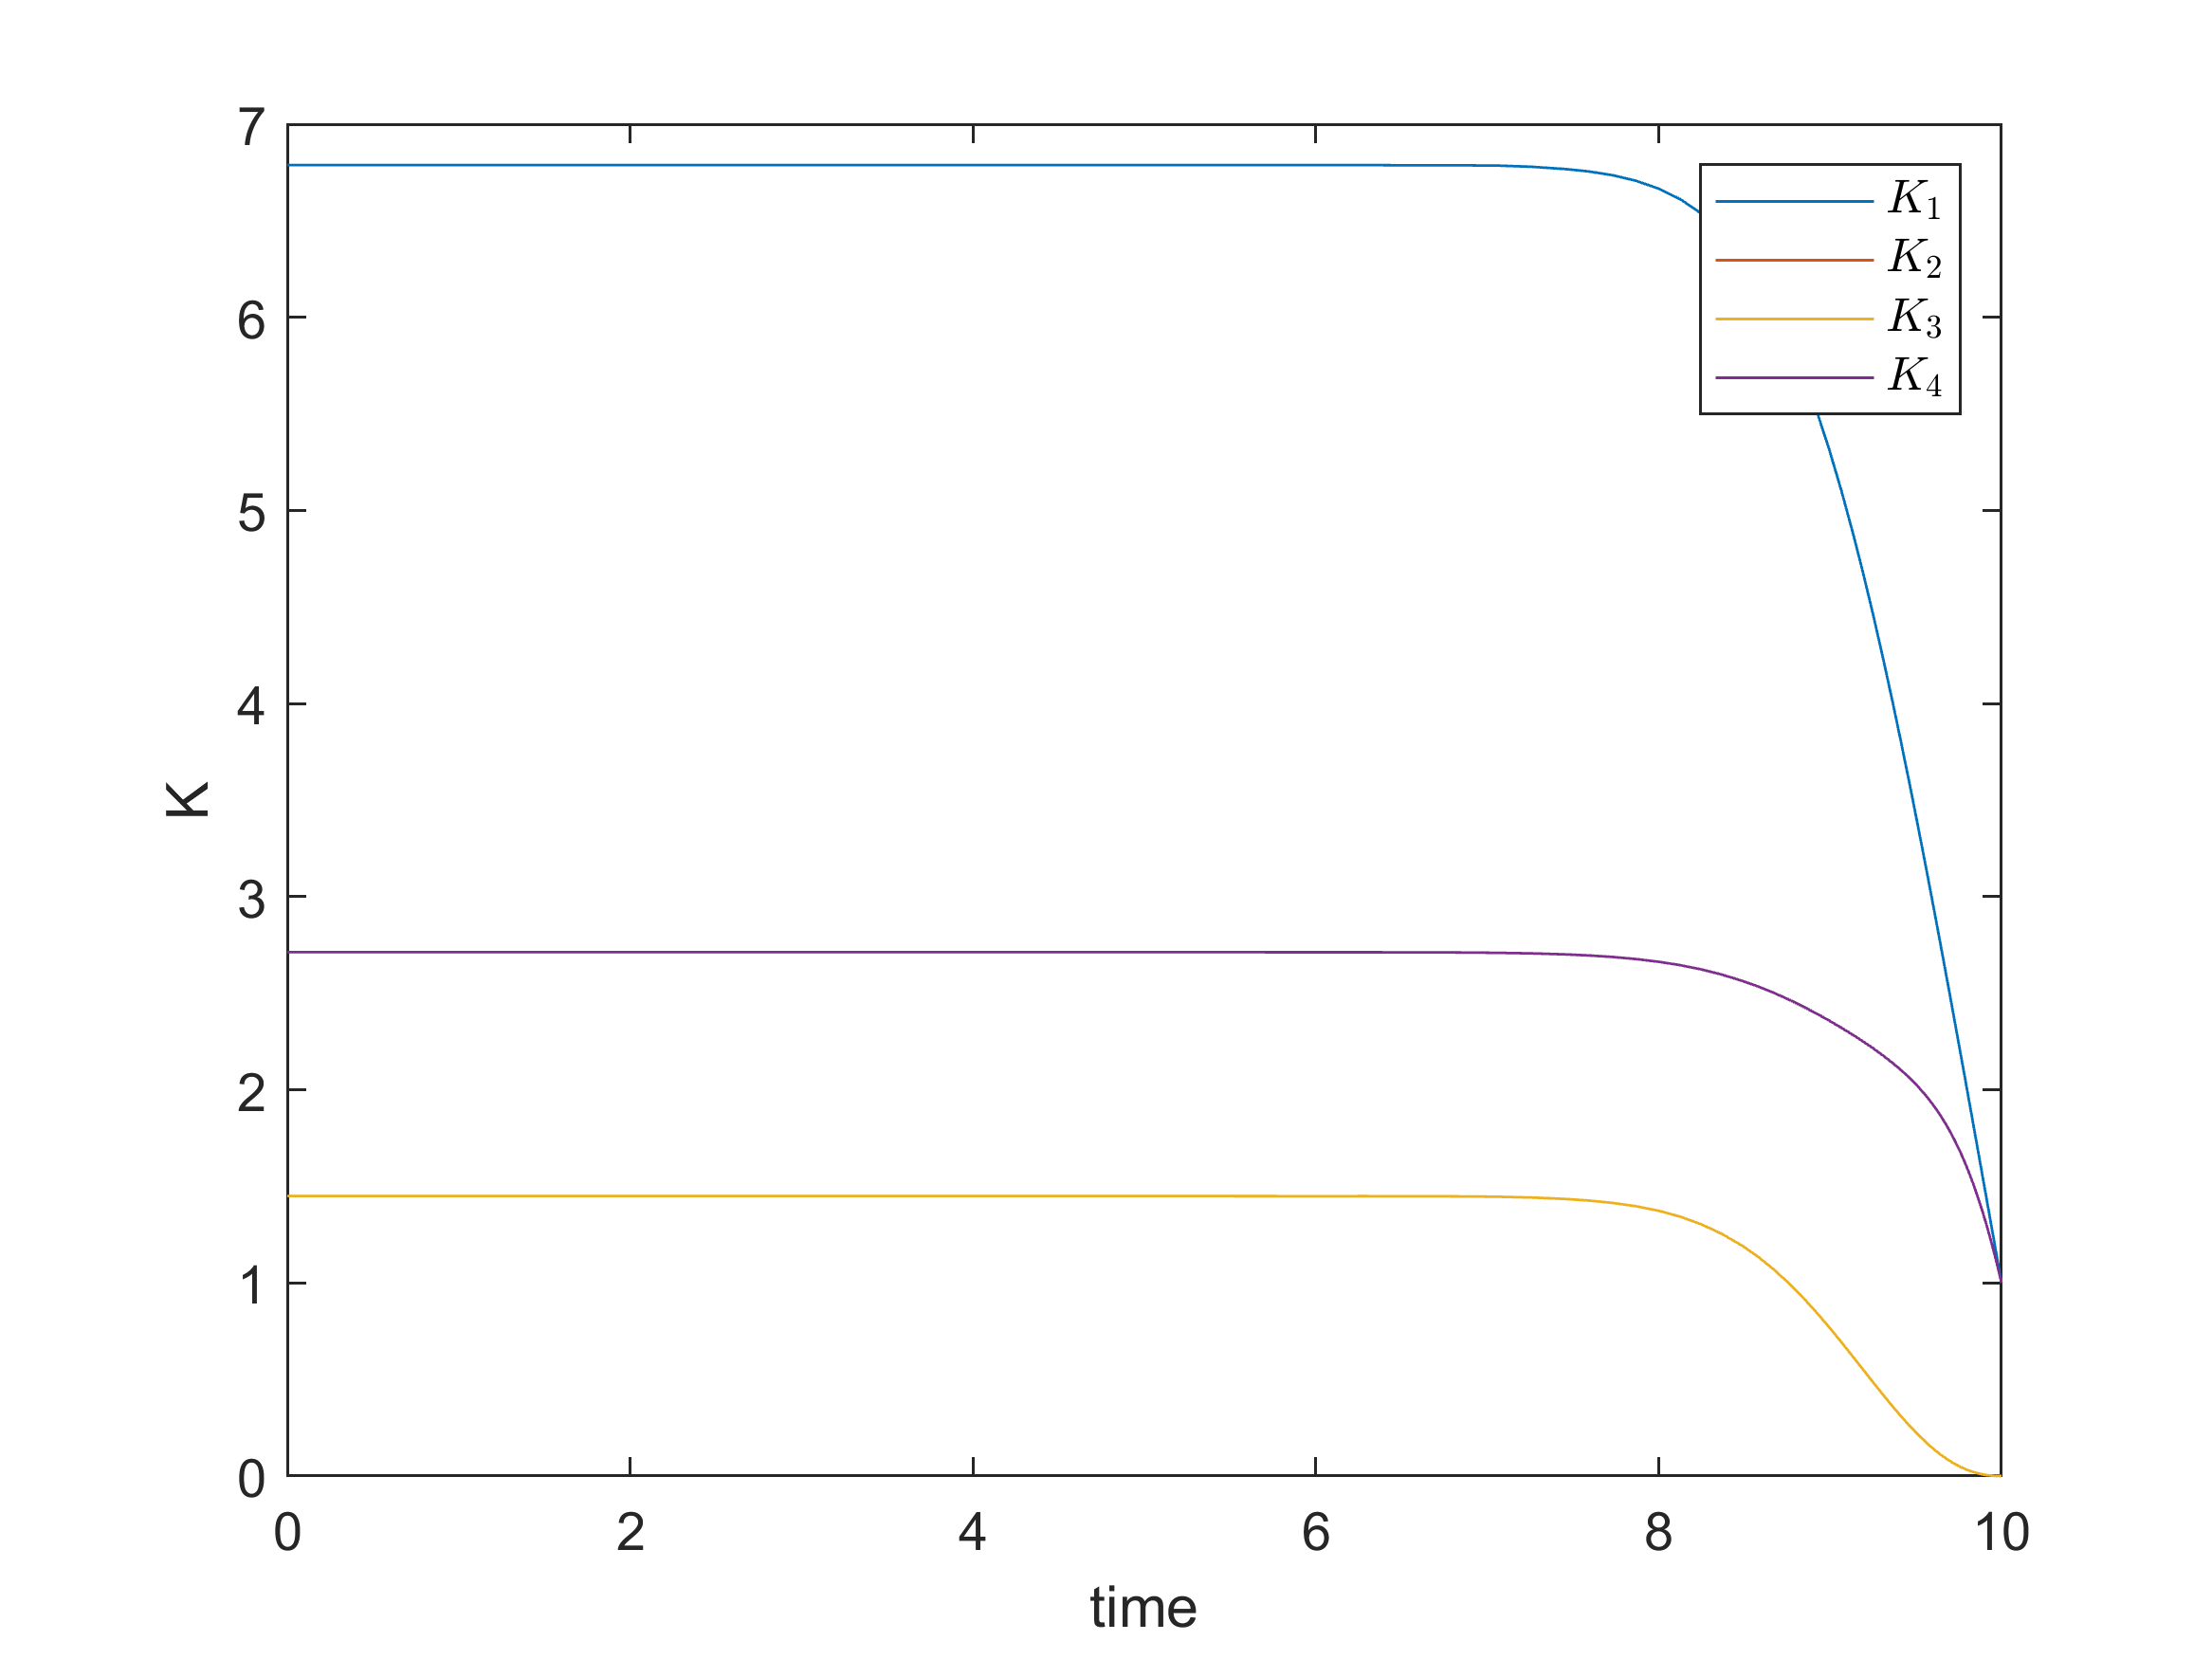
\includegraphics[width=12cm]{../Code/Q3/figures/Kalpha5.png}
\end{figure}
%%%%%%% u(t) %%%%%%%
\begin{figure}[H]
	\caption{$u(t)$ in $\alpha = 5$}
	\centering
	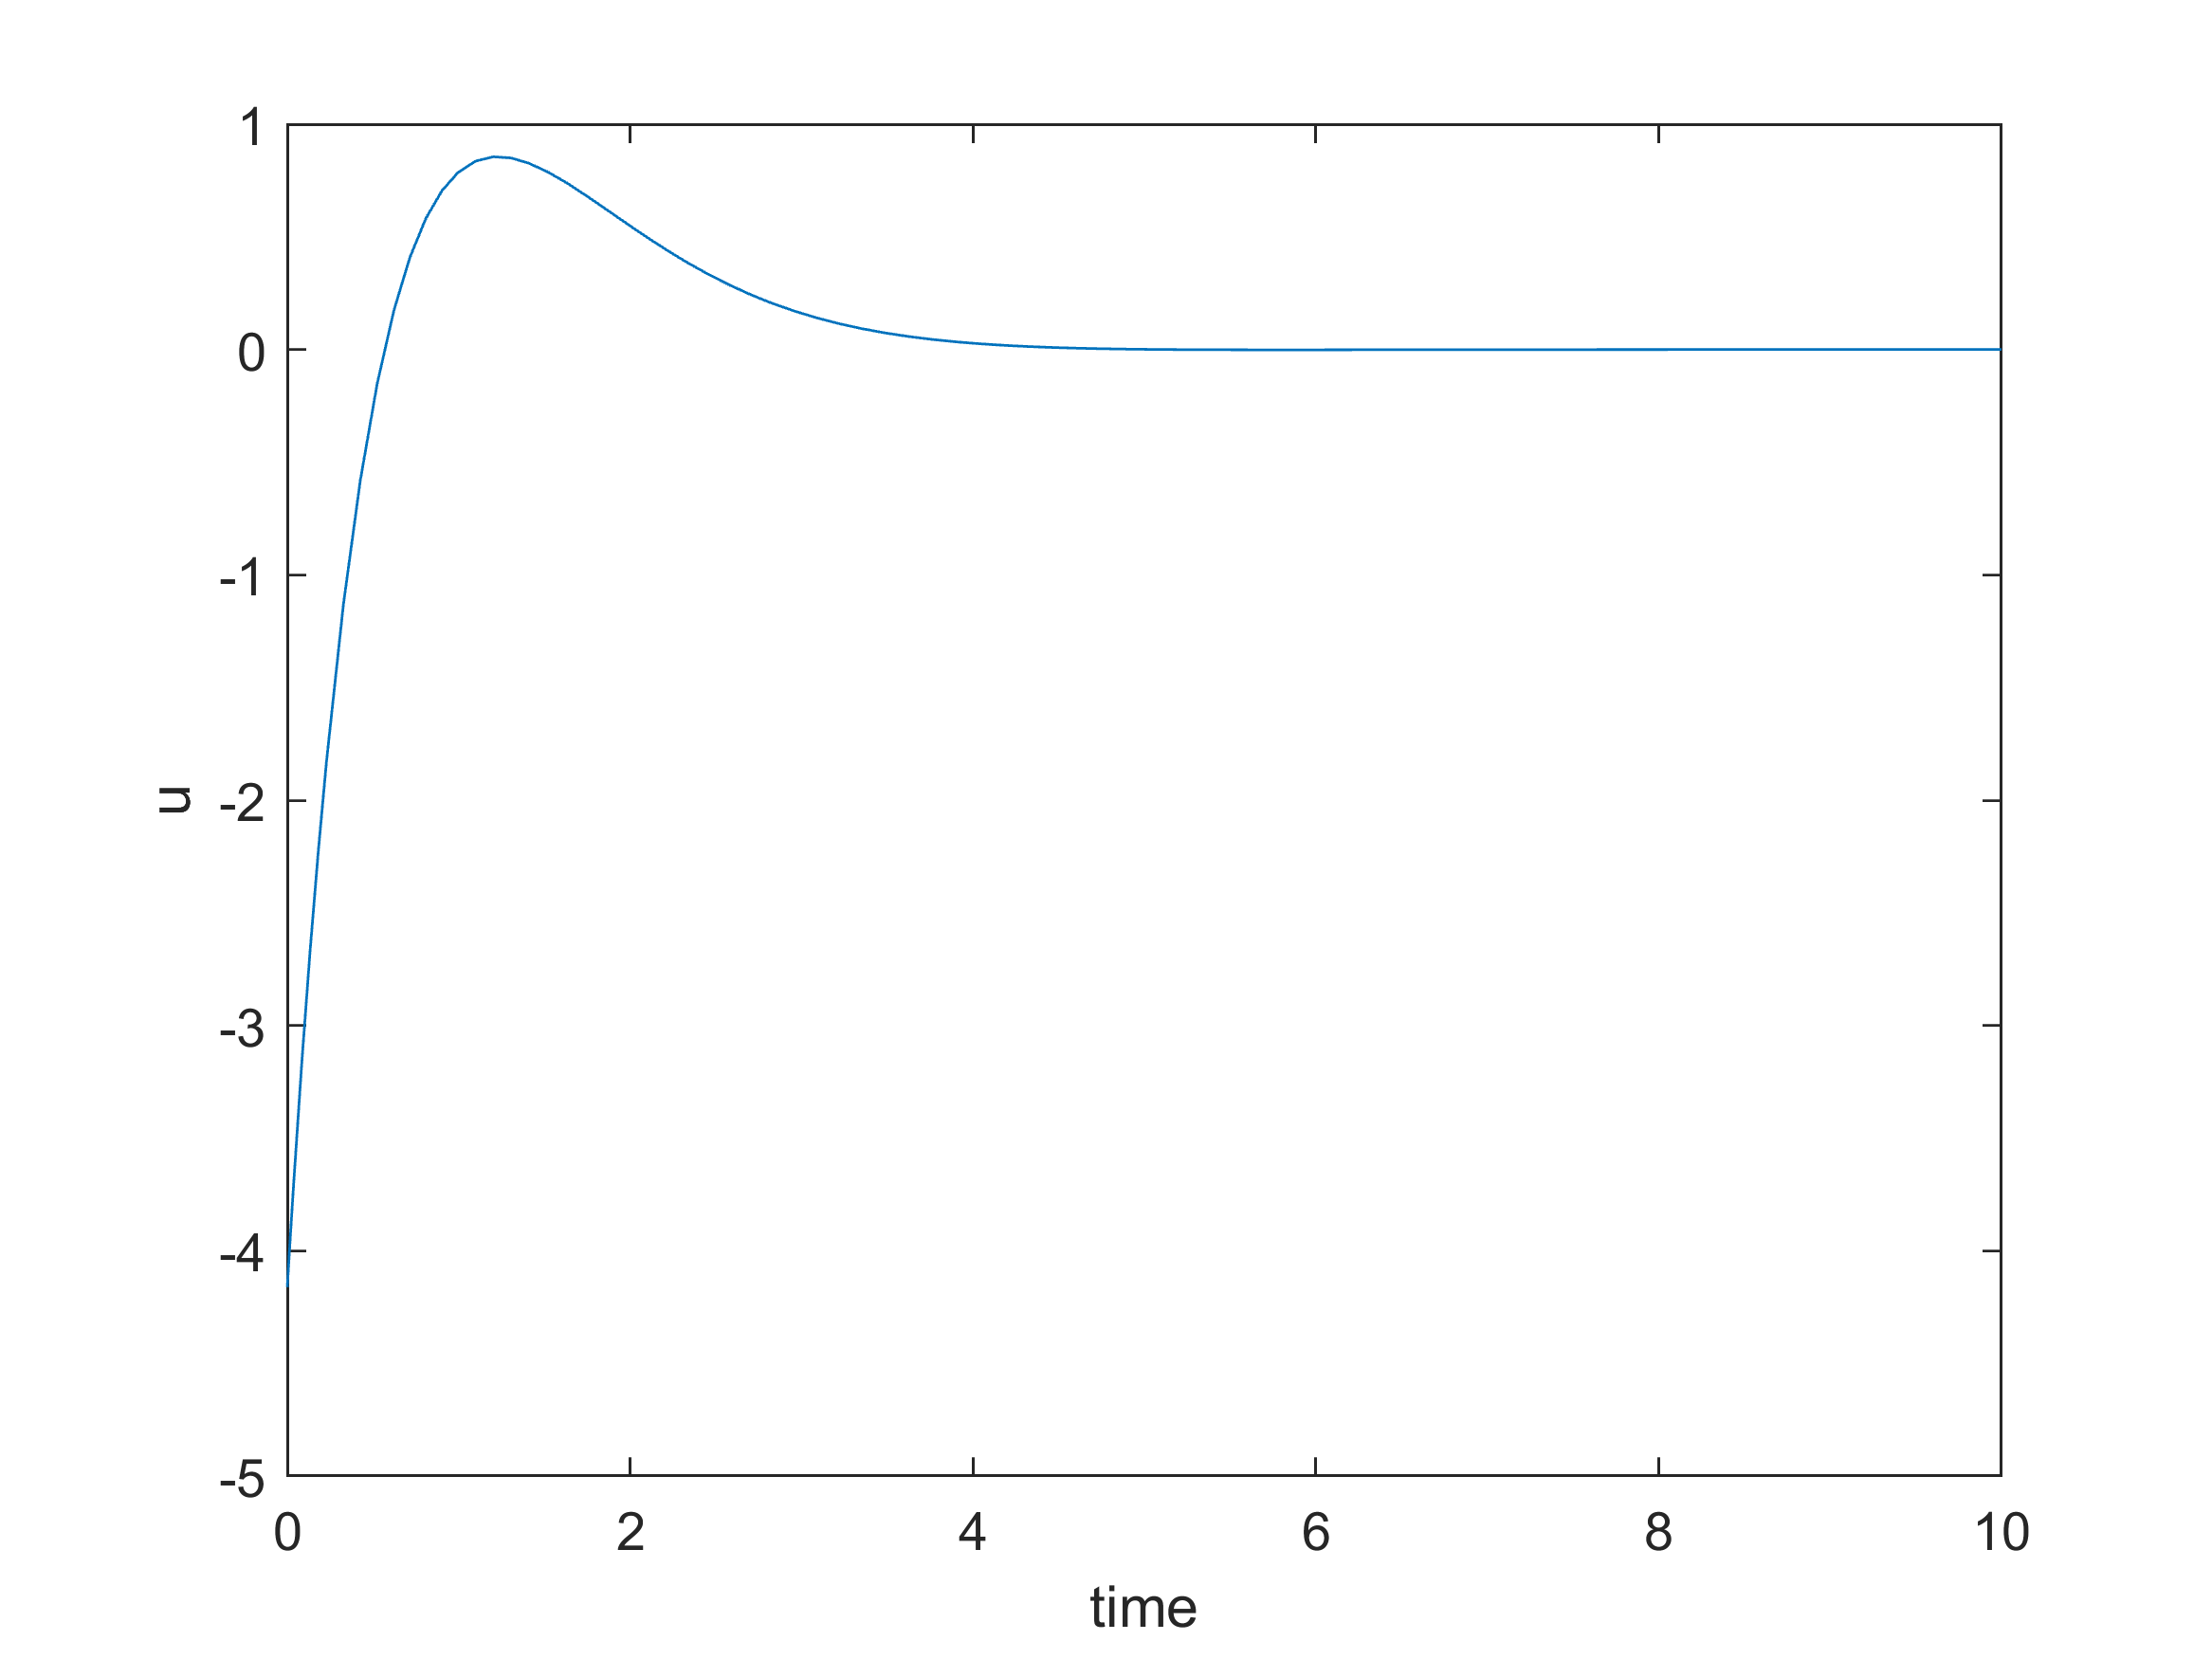
\includegraphics[width=12cm]{../Code/Q3/figures/ualpha5.png}
\end{figure}
%%%%%%% x(t) %%%%%%%
\begin{figure}[H]
	\caption{System States $\vec x(t)$ in $\alpha = 5$}
	\centering
	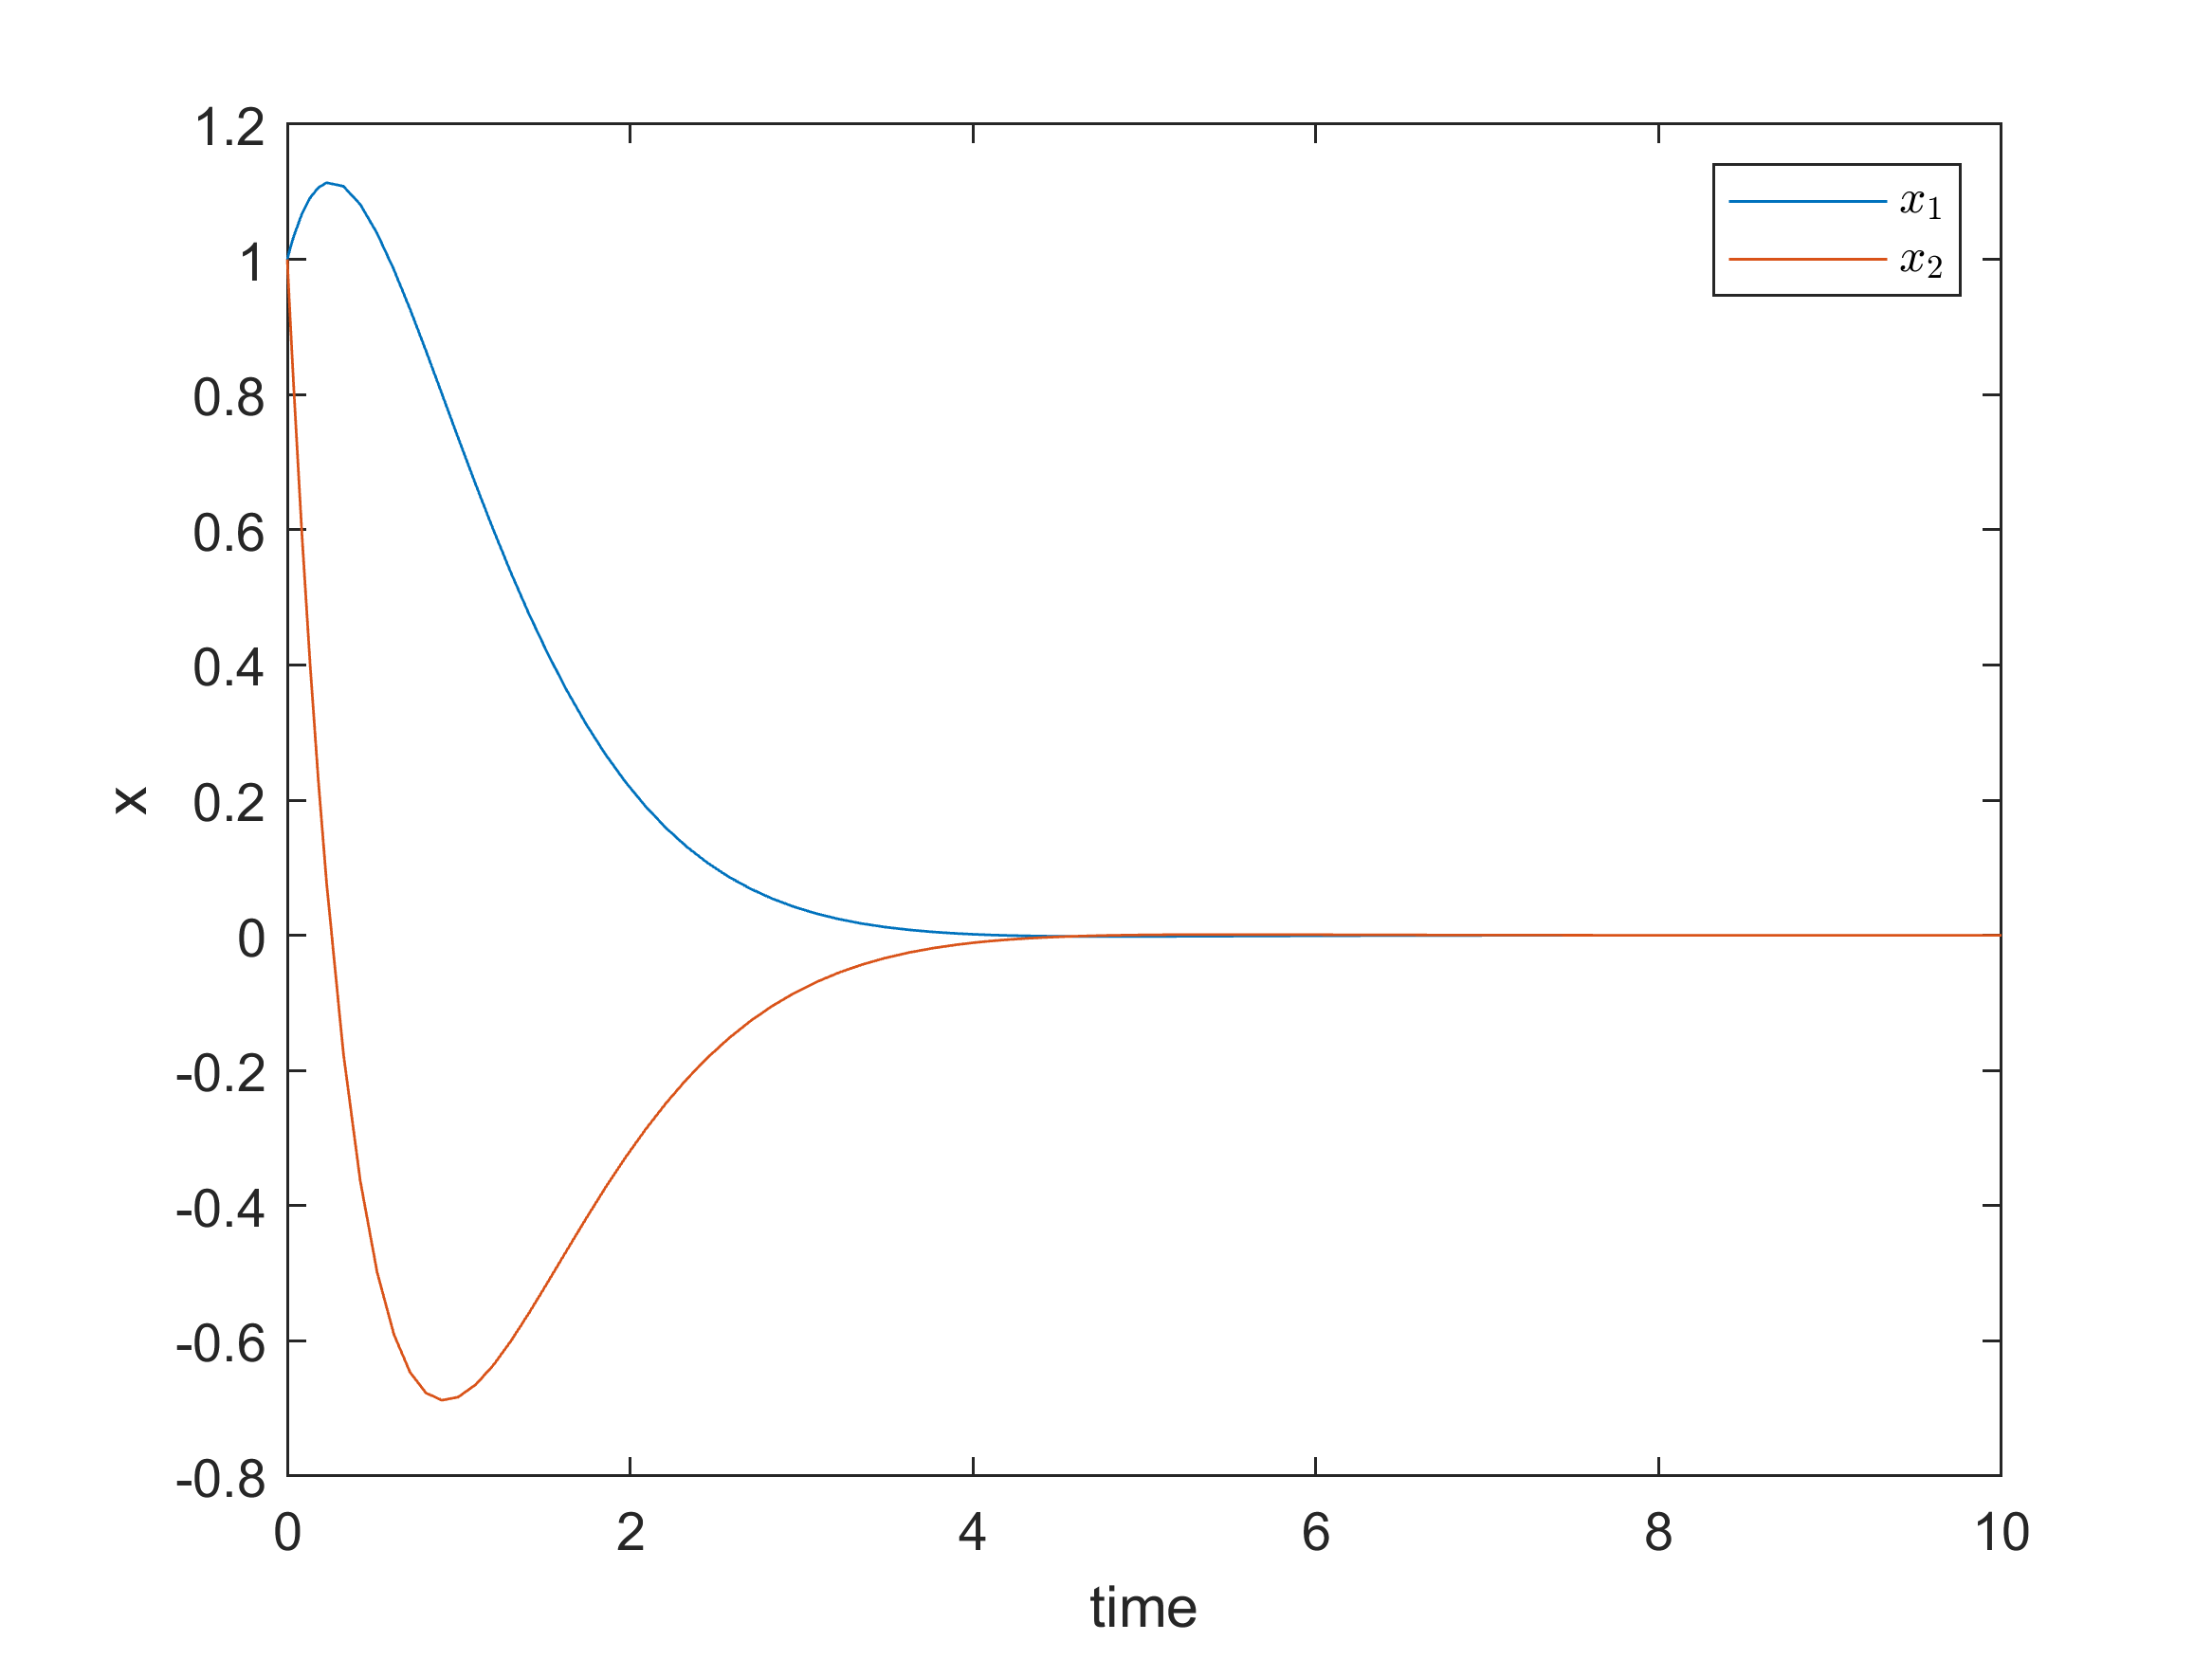
\includegraphics[width=12cm]{../Code/Q3/figures/xalpha5.png}
\end{figure}
	%%%%%%%%% alpha = 10 %%%%%%%%%
\item $\alpha = 10$
%%%%%%% K(t) %%%%%%%
\begin{figure}[H]
	\caption{$K(t)$ in $\alpha = 10$}
	\centering
	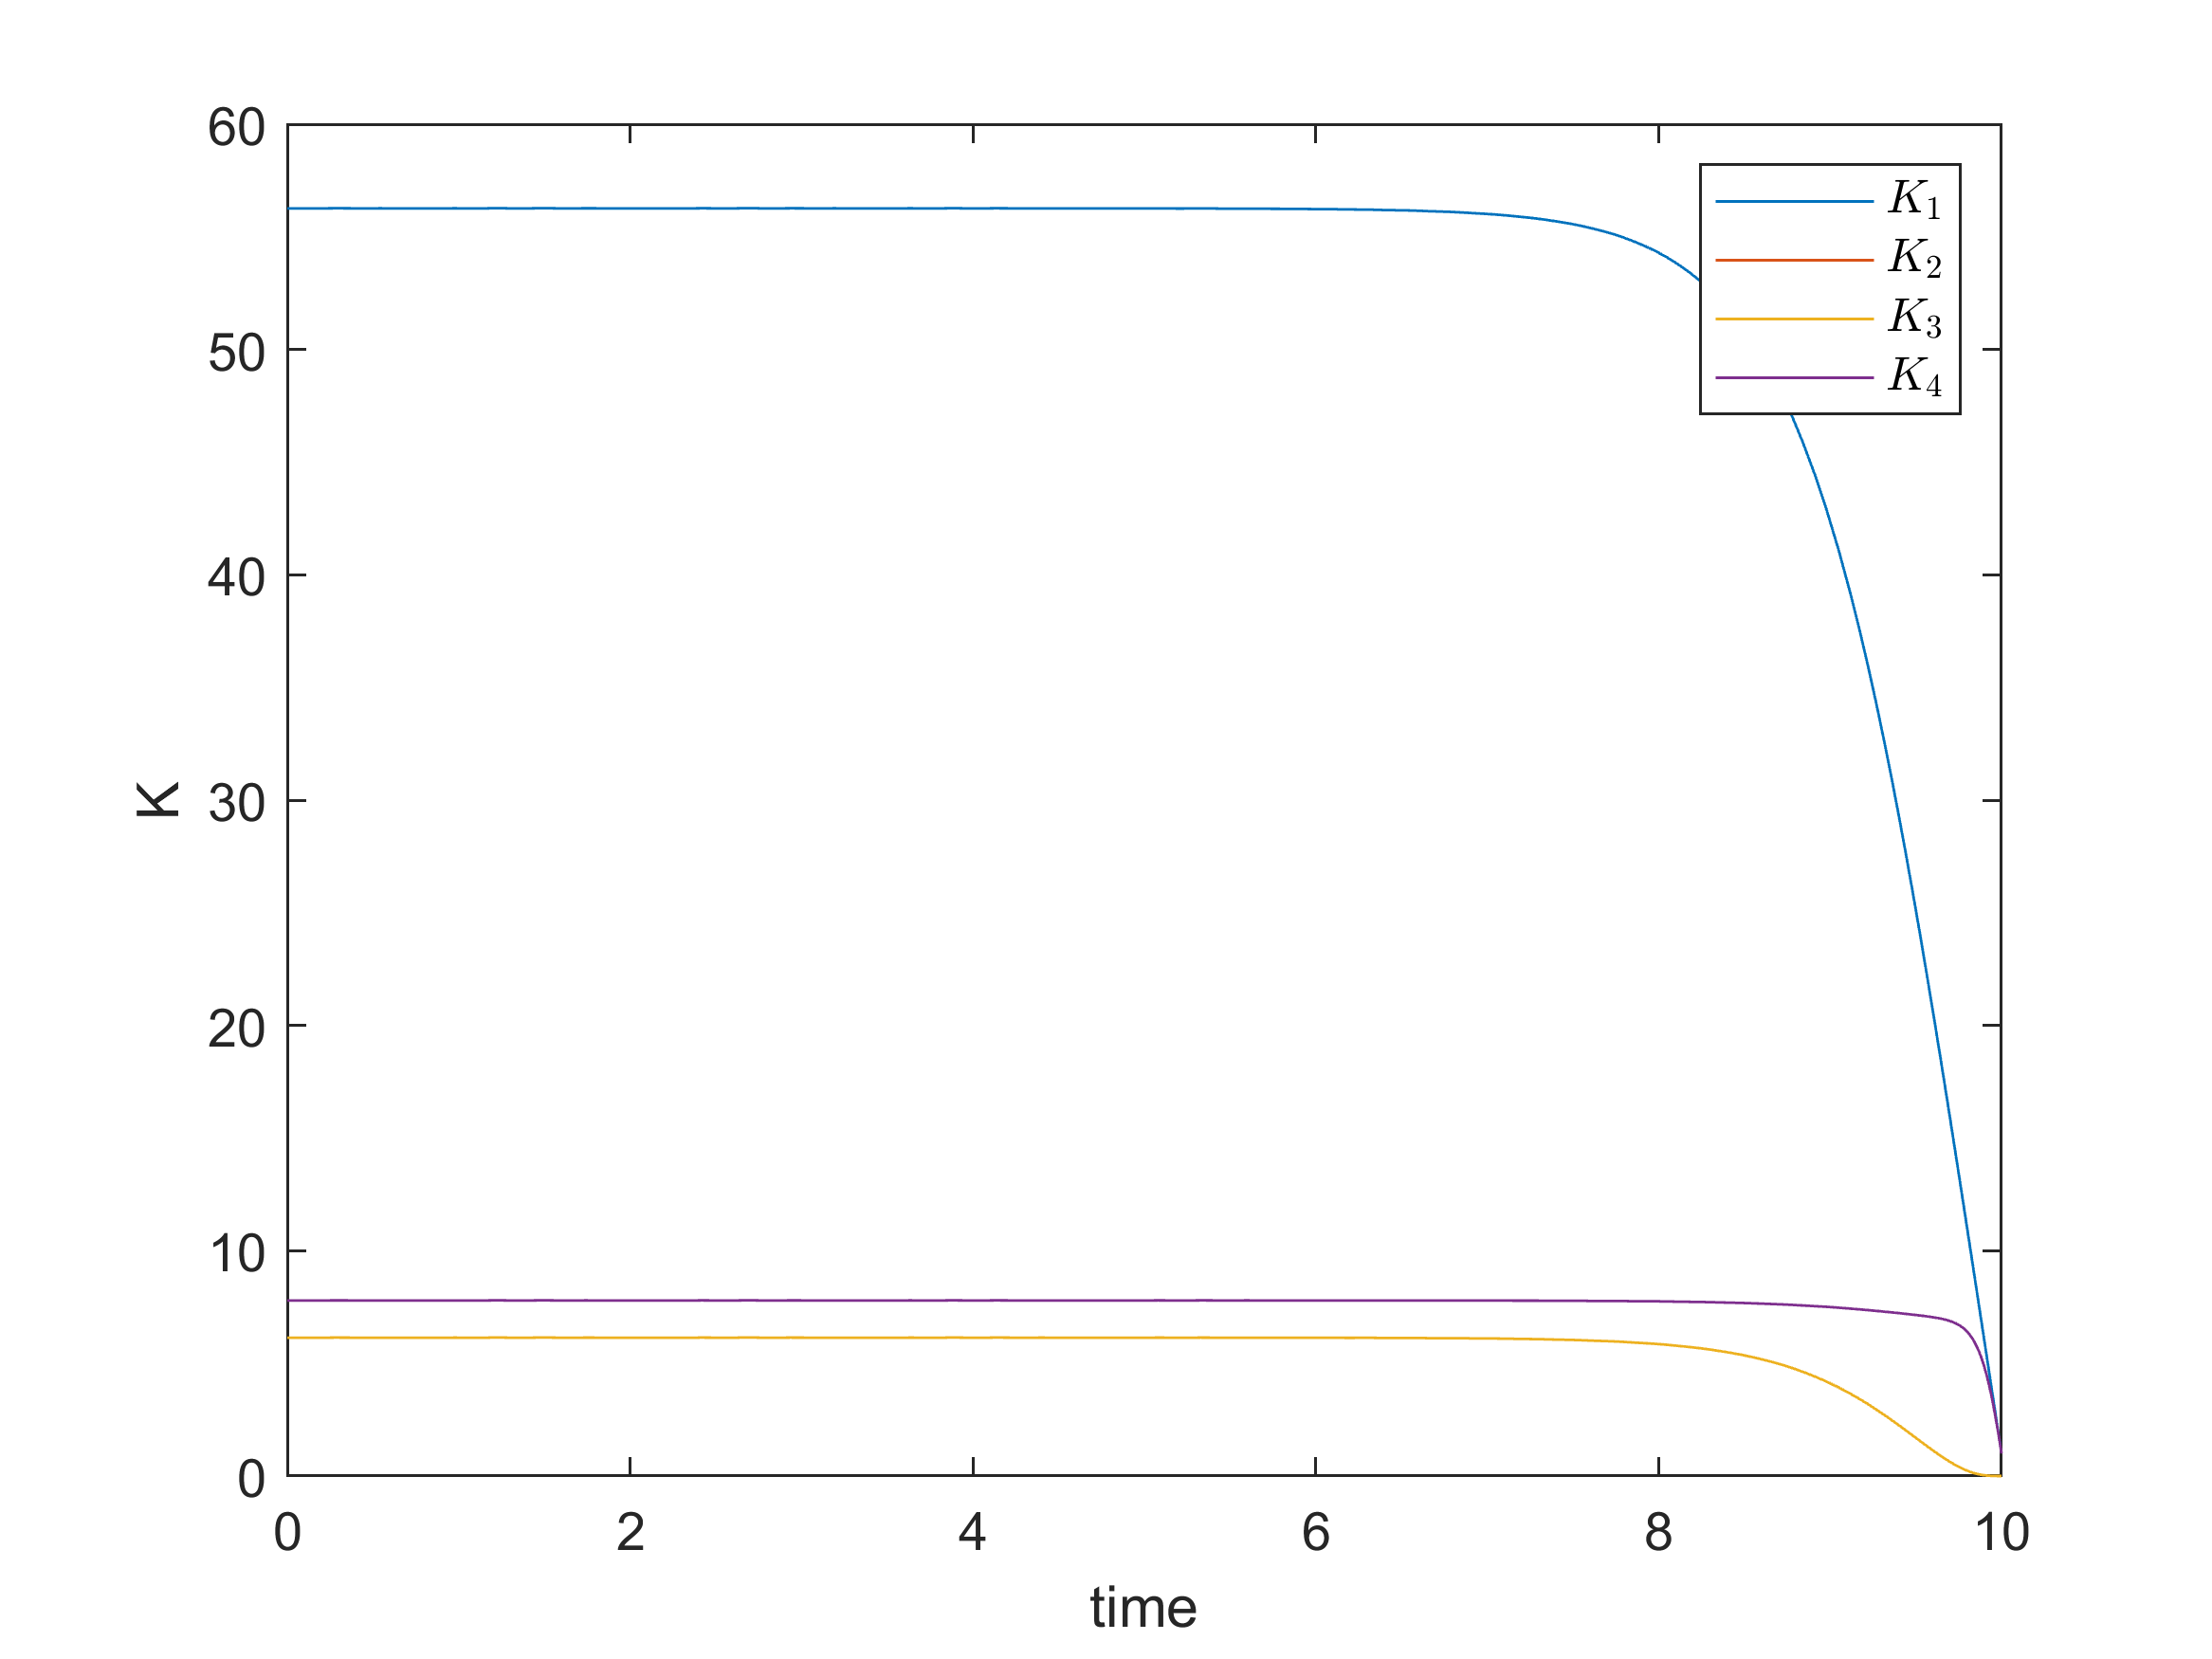
\includegraphics[width=12cm]{../Code/Q3/figures/Kalpha10.png}
\end{figure}
%%%%%%% u(t) %%%%%%%
\begin{figure}[H]
	\caption{$u(t)$ in $\alpha = 10$}
	\centering
	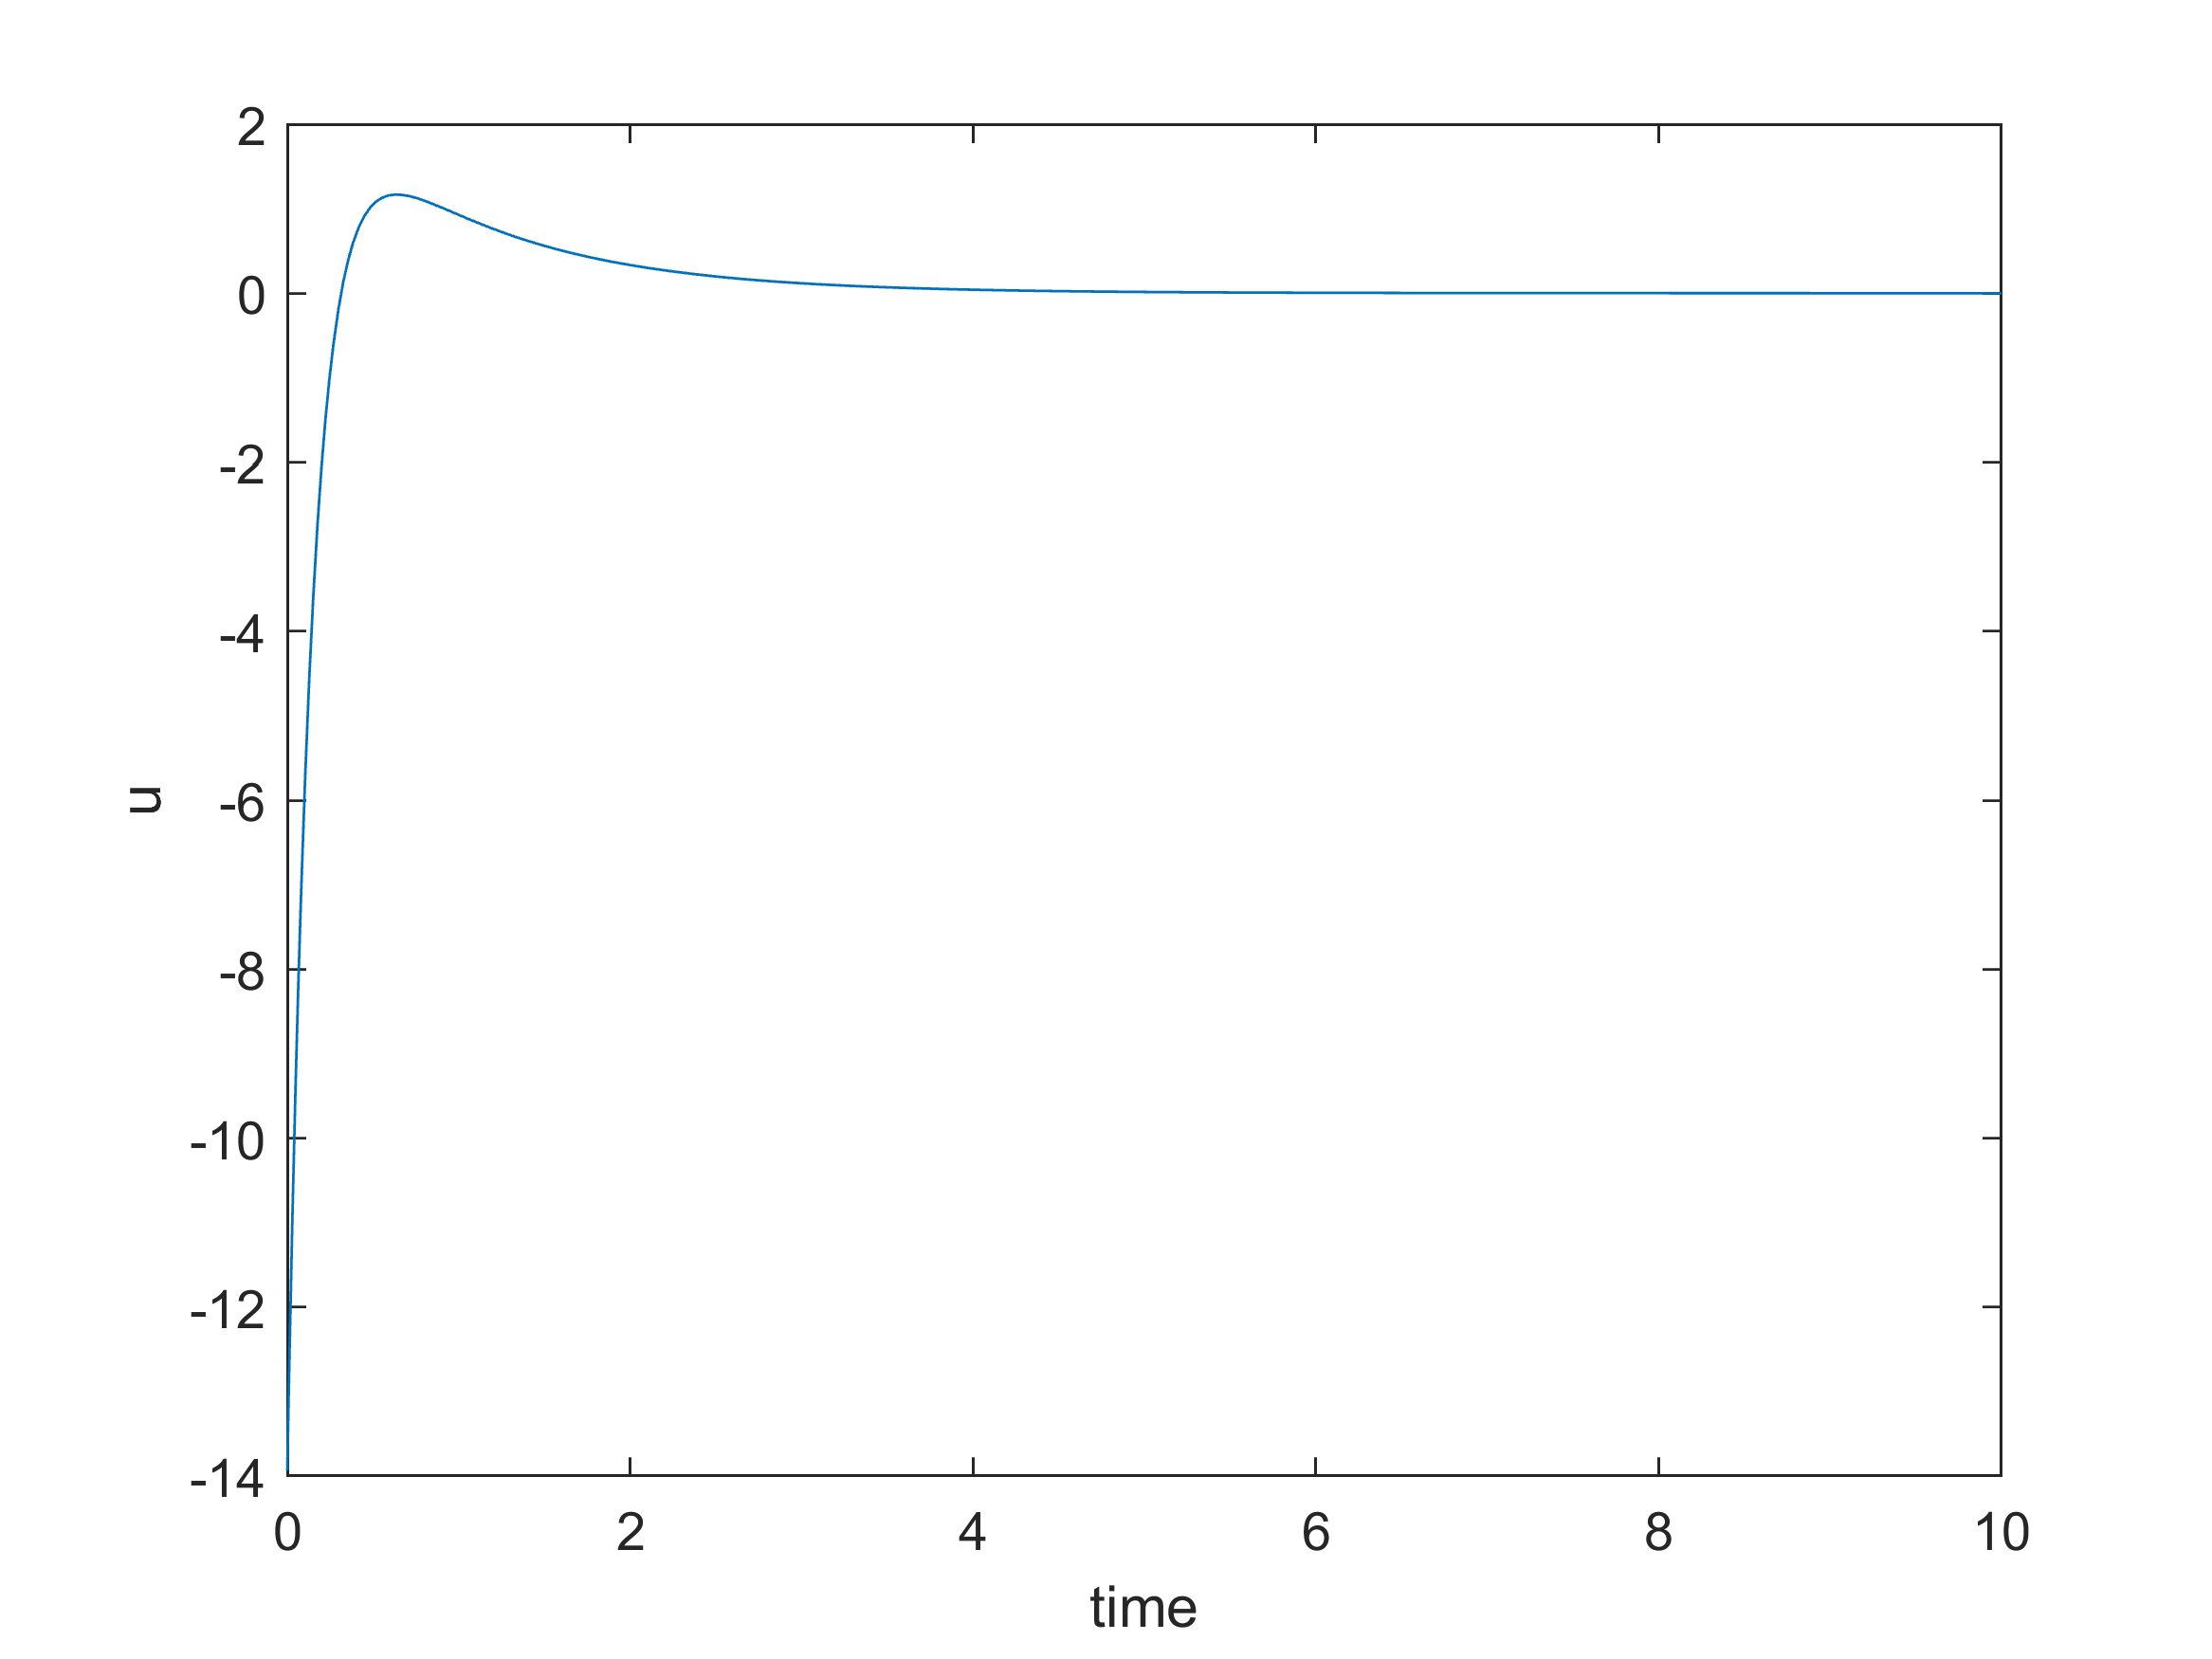
\includegraphics[width=12cm]{../Code/Q3/figures/ualpha10.png}
\end{figure}
%%%%%%% x(t) %%%%%%%
\begin{figure}[H]
	\caption{System States $\vec x(t)$ in $\alpha = 10$}
	\centering
	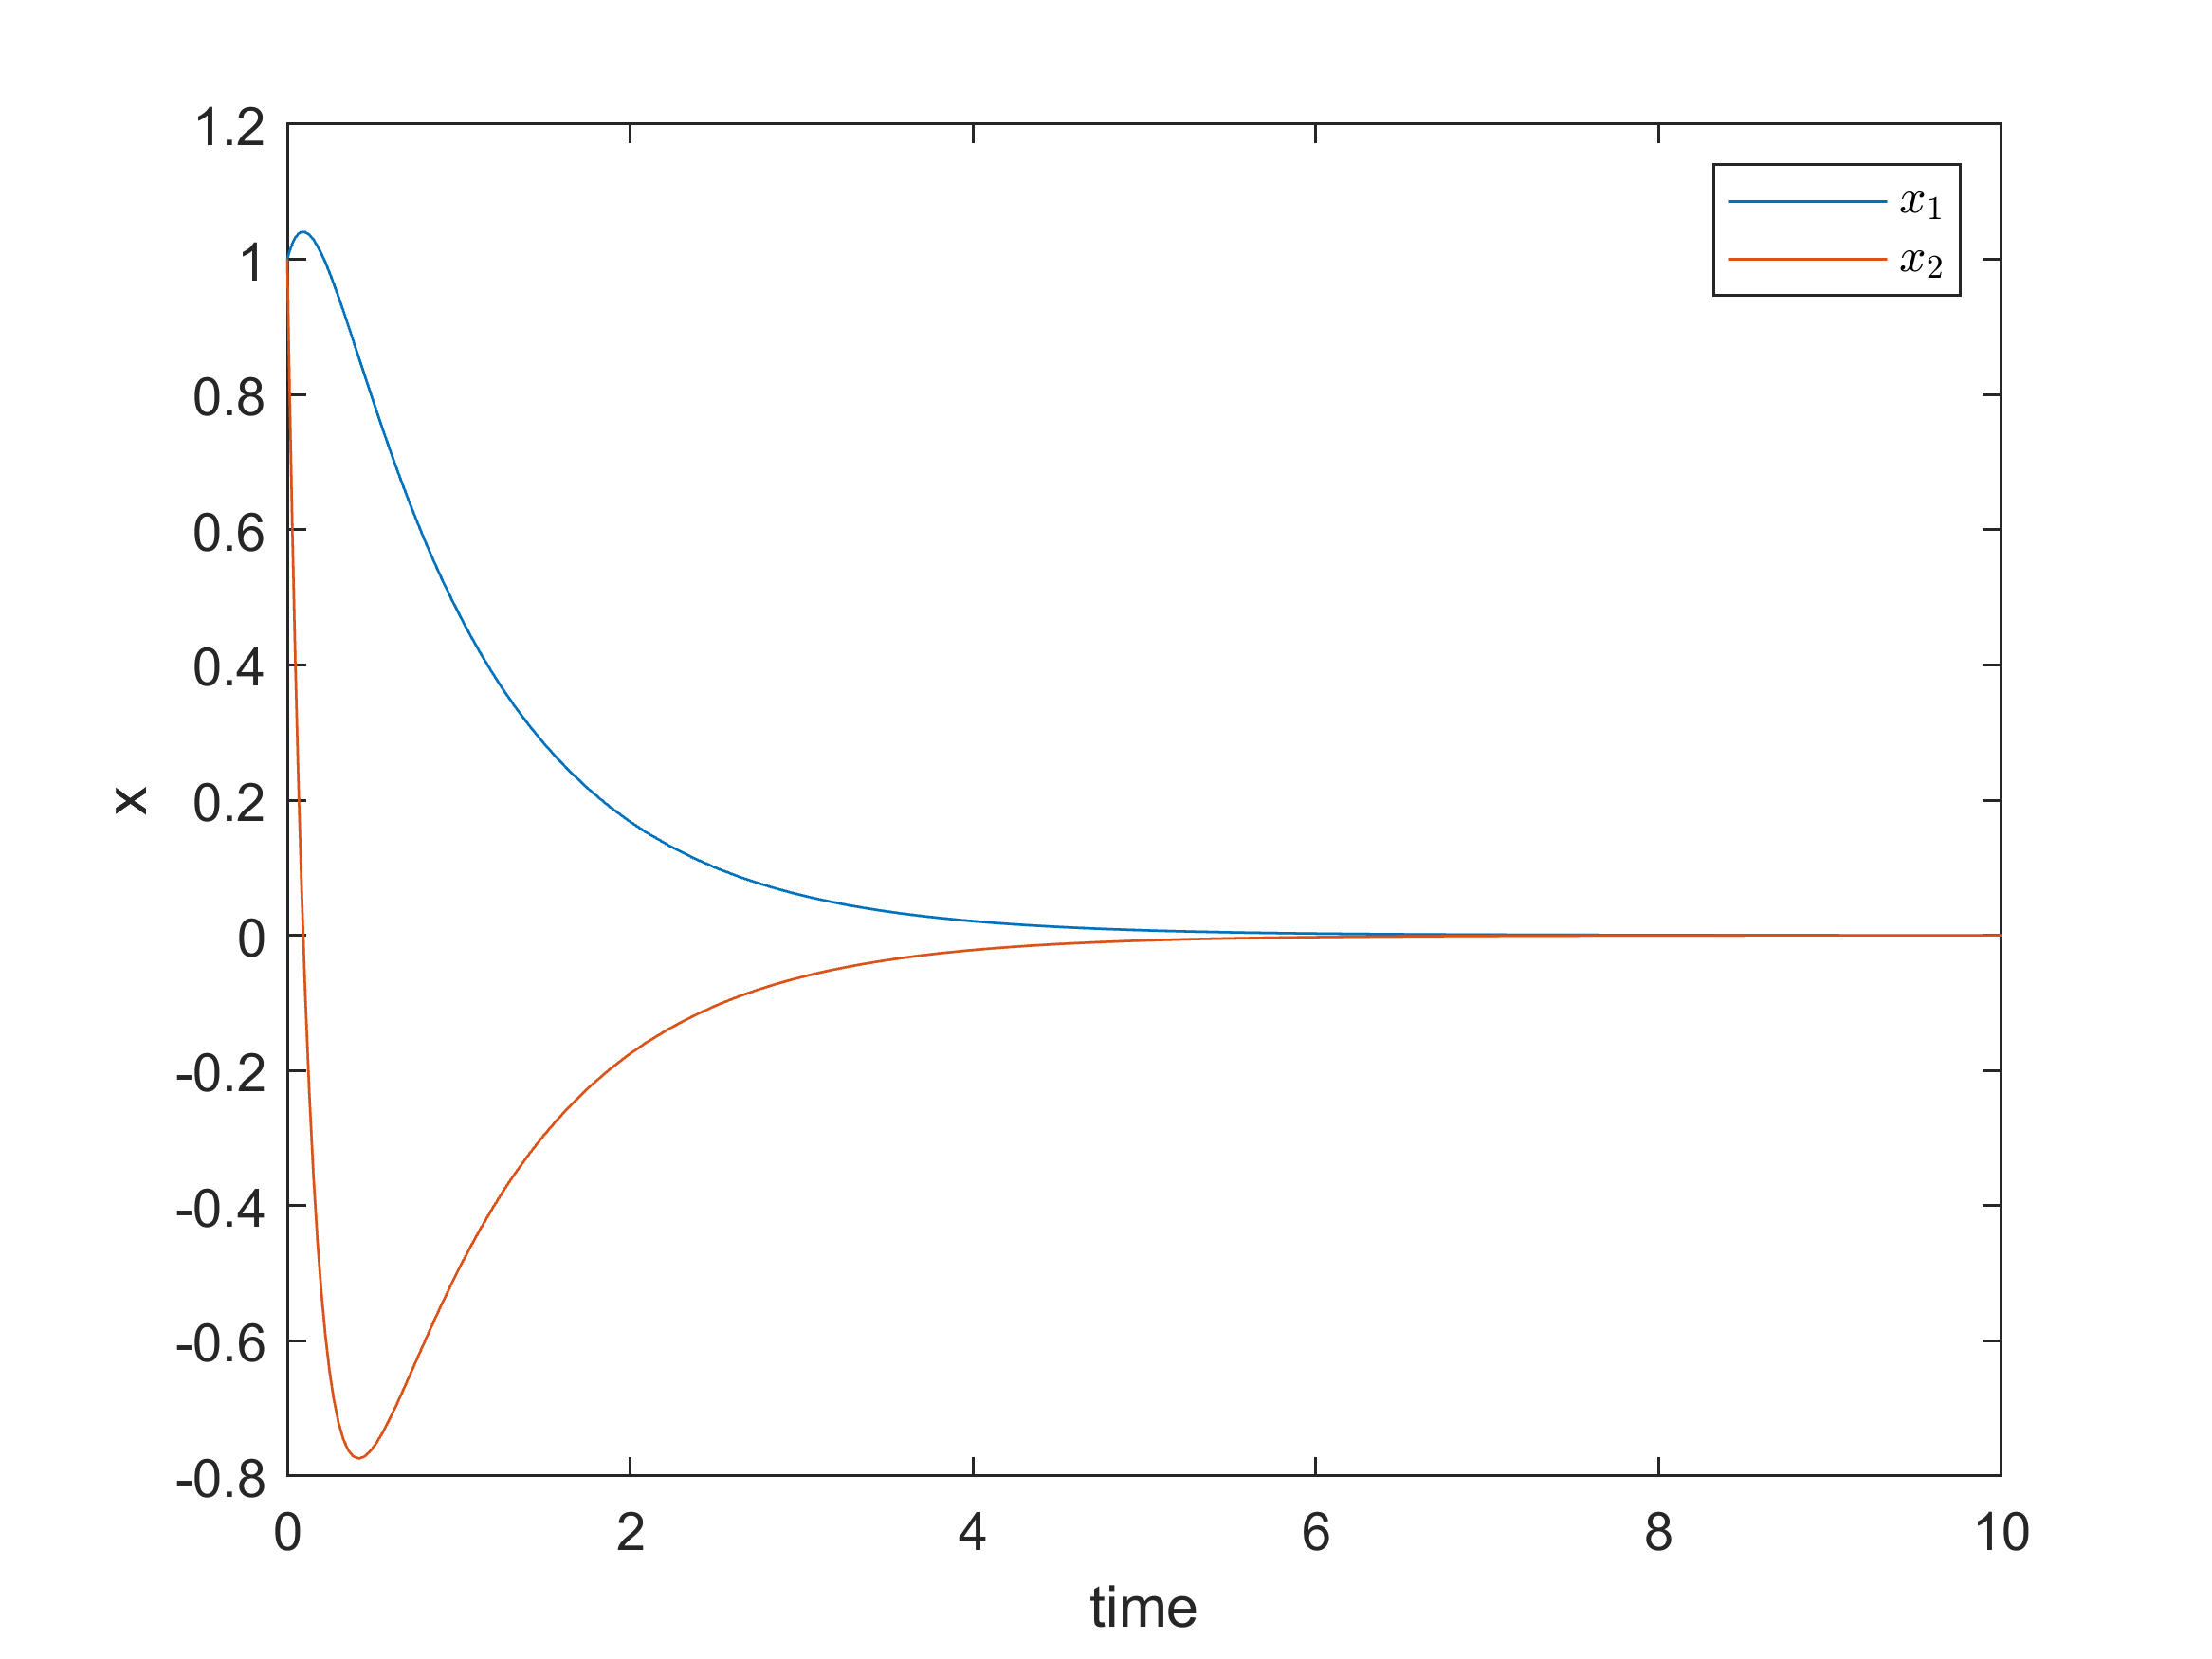
\includegraphics[width=12cm]{../Code/Q3/figures/xalpha10.png}
\end{figure}
%%%%%%%%% K(t) sub plot %%%%%%%%%
\item $K(t)$ for all simulated $\alpha$
\begin{figure}[H]
	\caption{$K(t)$ for all simulated $\alpha$}
	\centering
	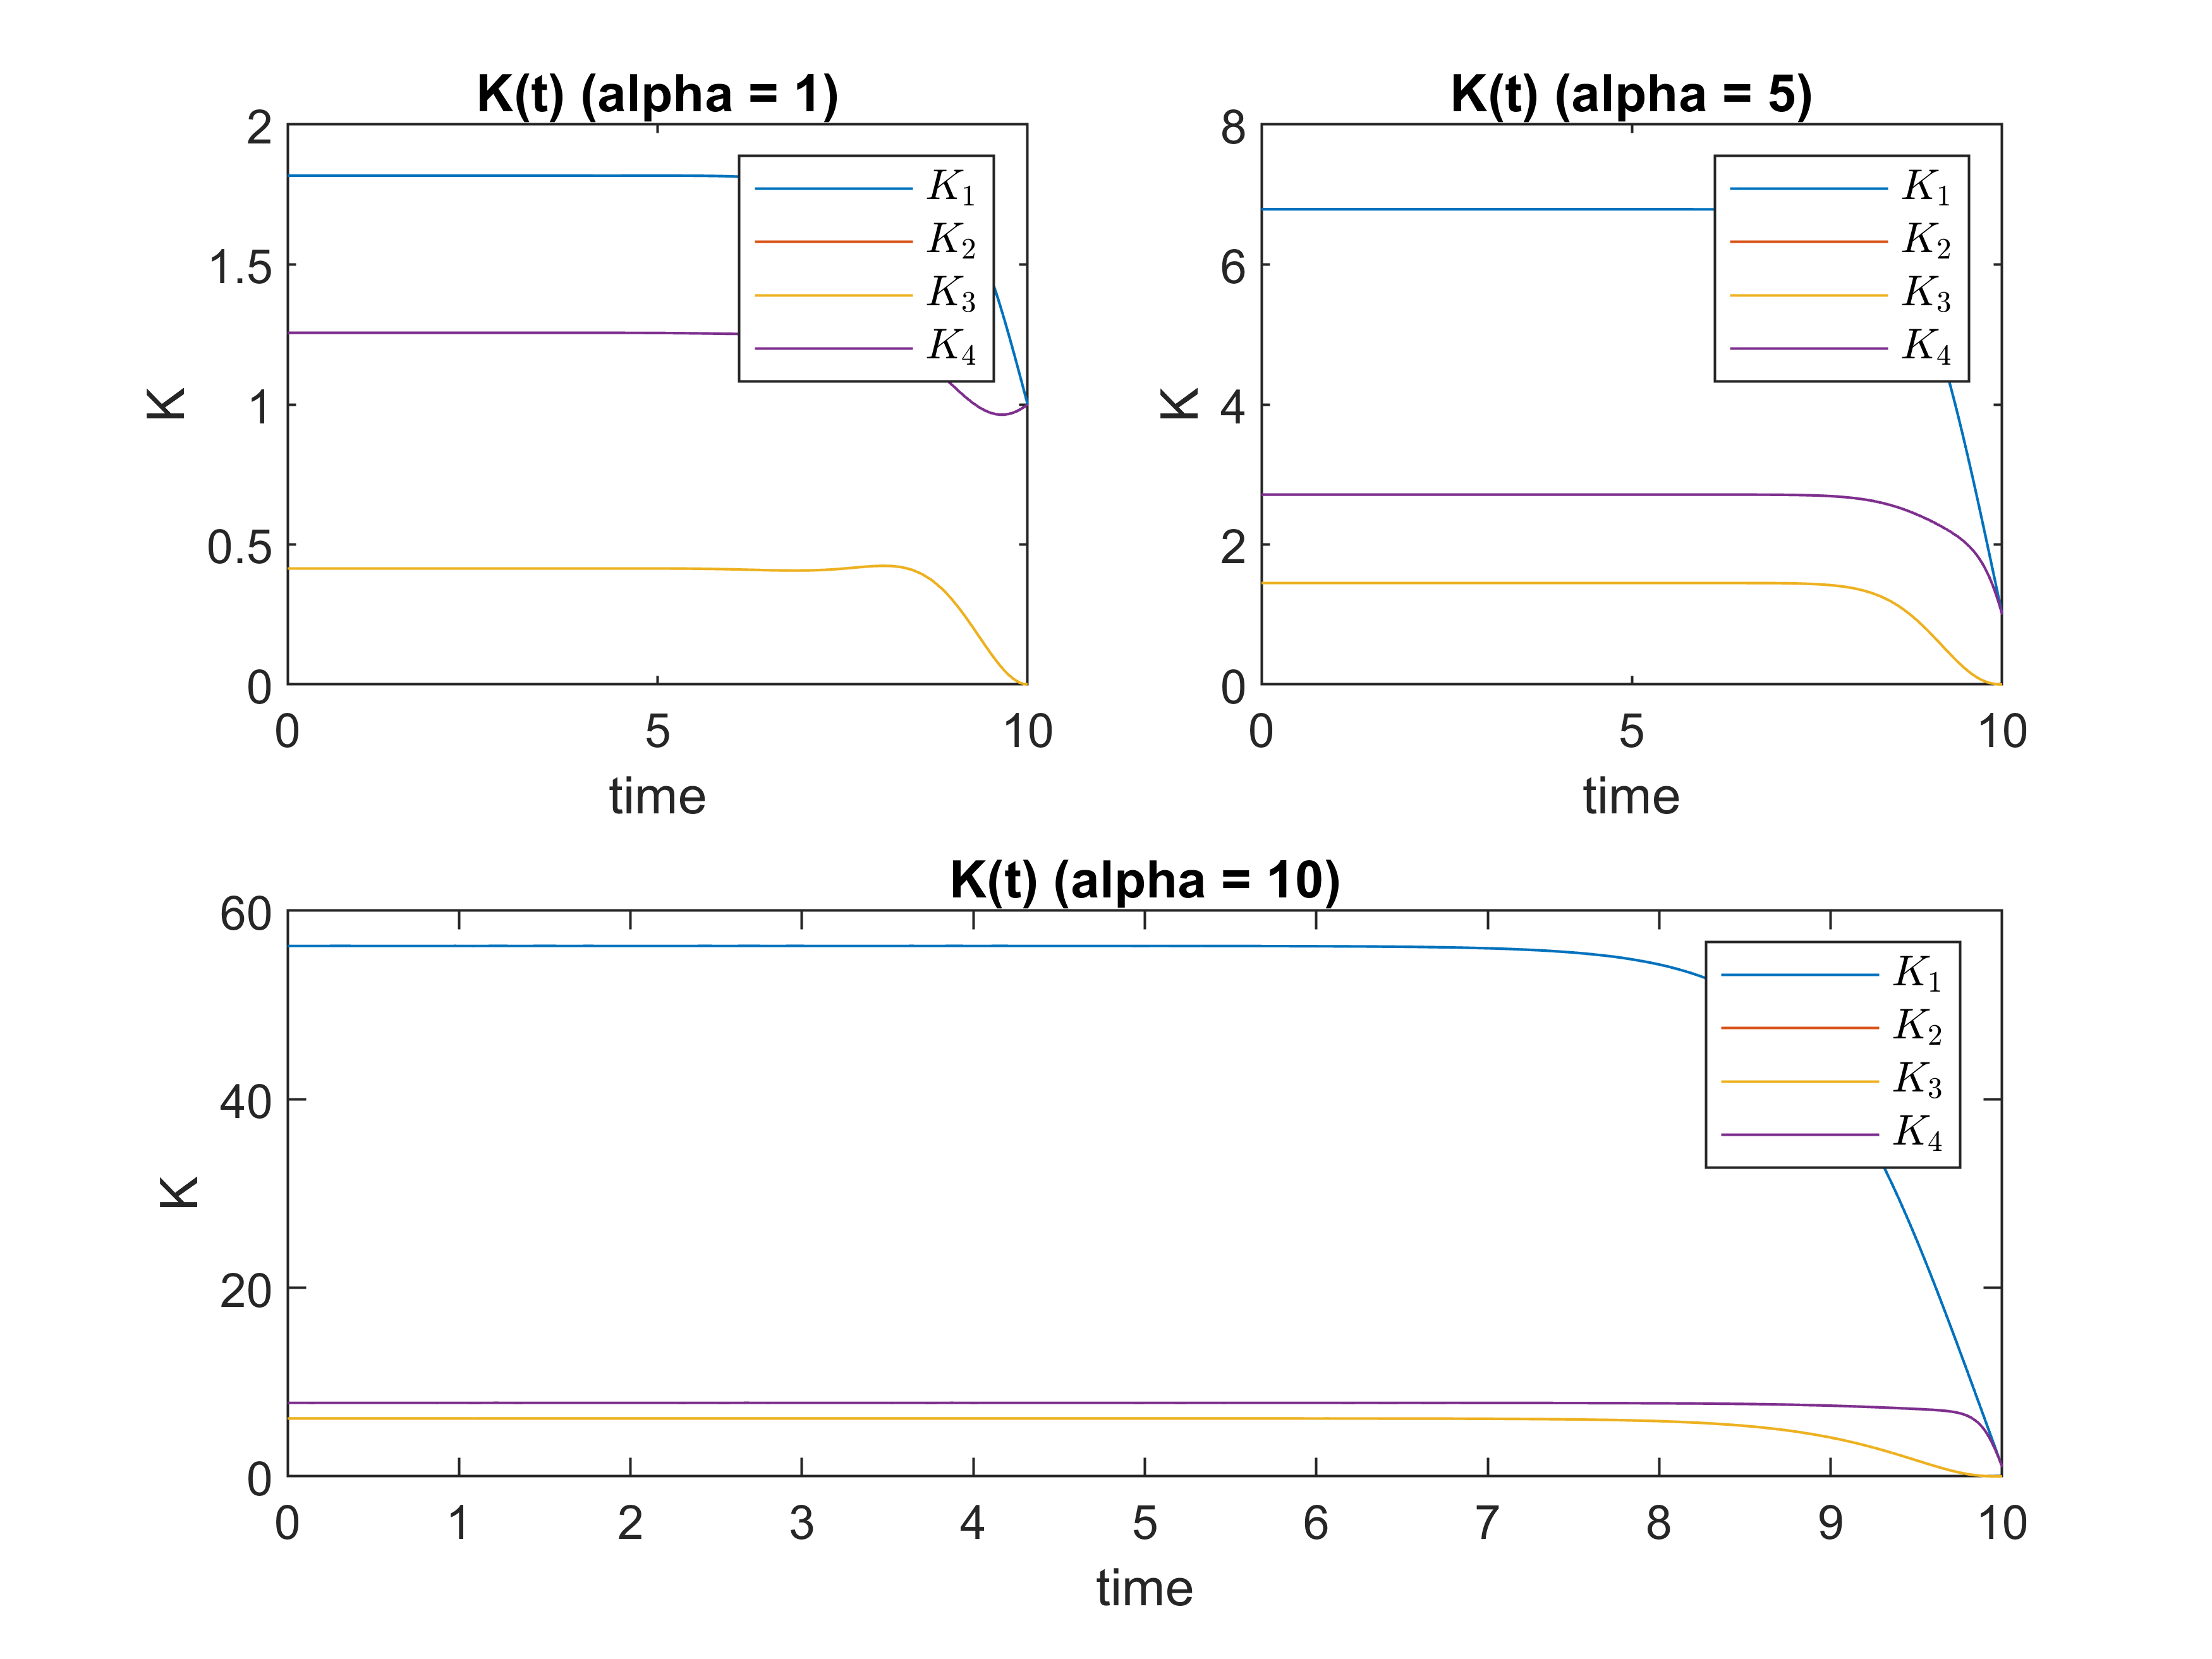
\includegraphics[width=12cm]{../Code/Q3/figures/SubplotQ3_dK.png}
\end{figure}
%%%%%%%%% u(t) sub plot %%%%%%%%%
\item $u(t)$ for all simulated $\alpha$
\begin{figure}[H]
	\caption{$u(t)$ for all simulated $\alpha$}
	\centering
	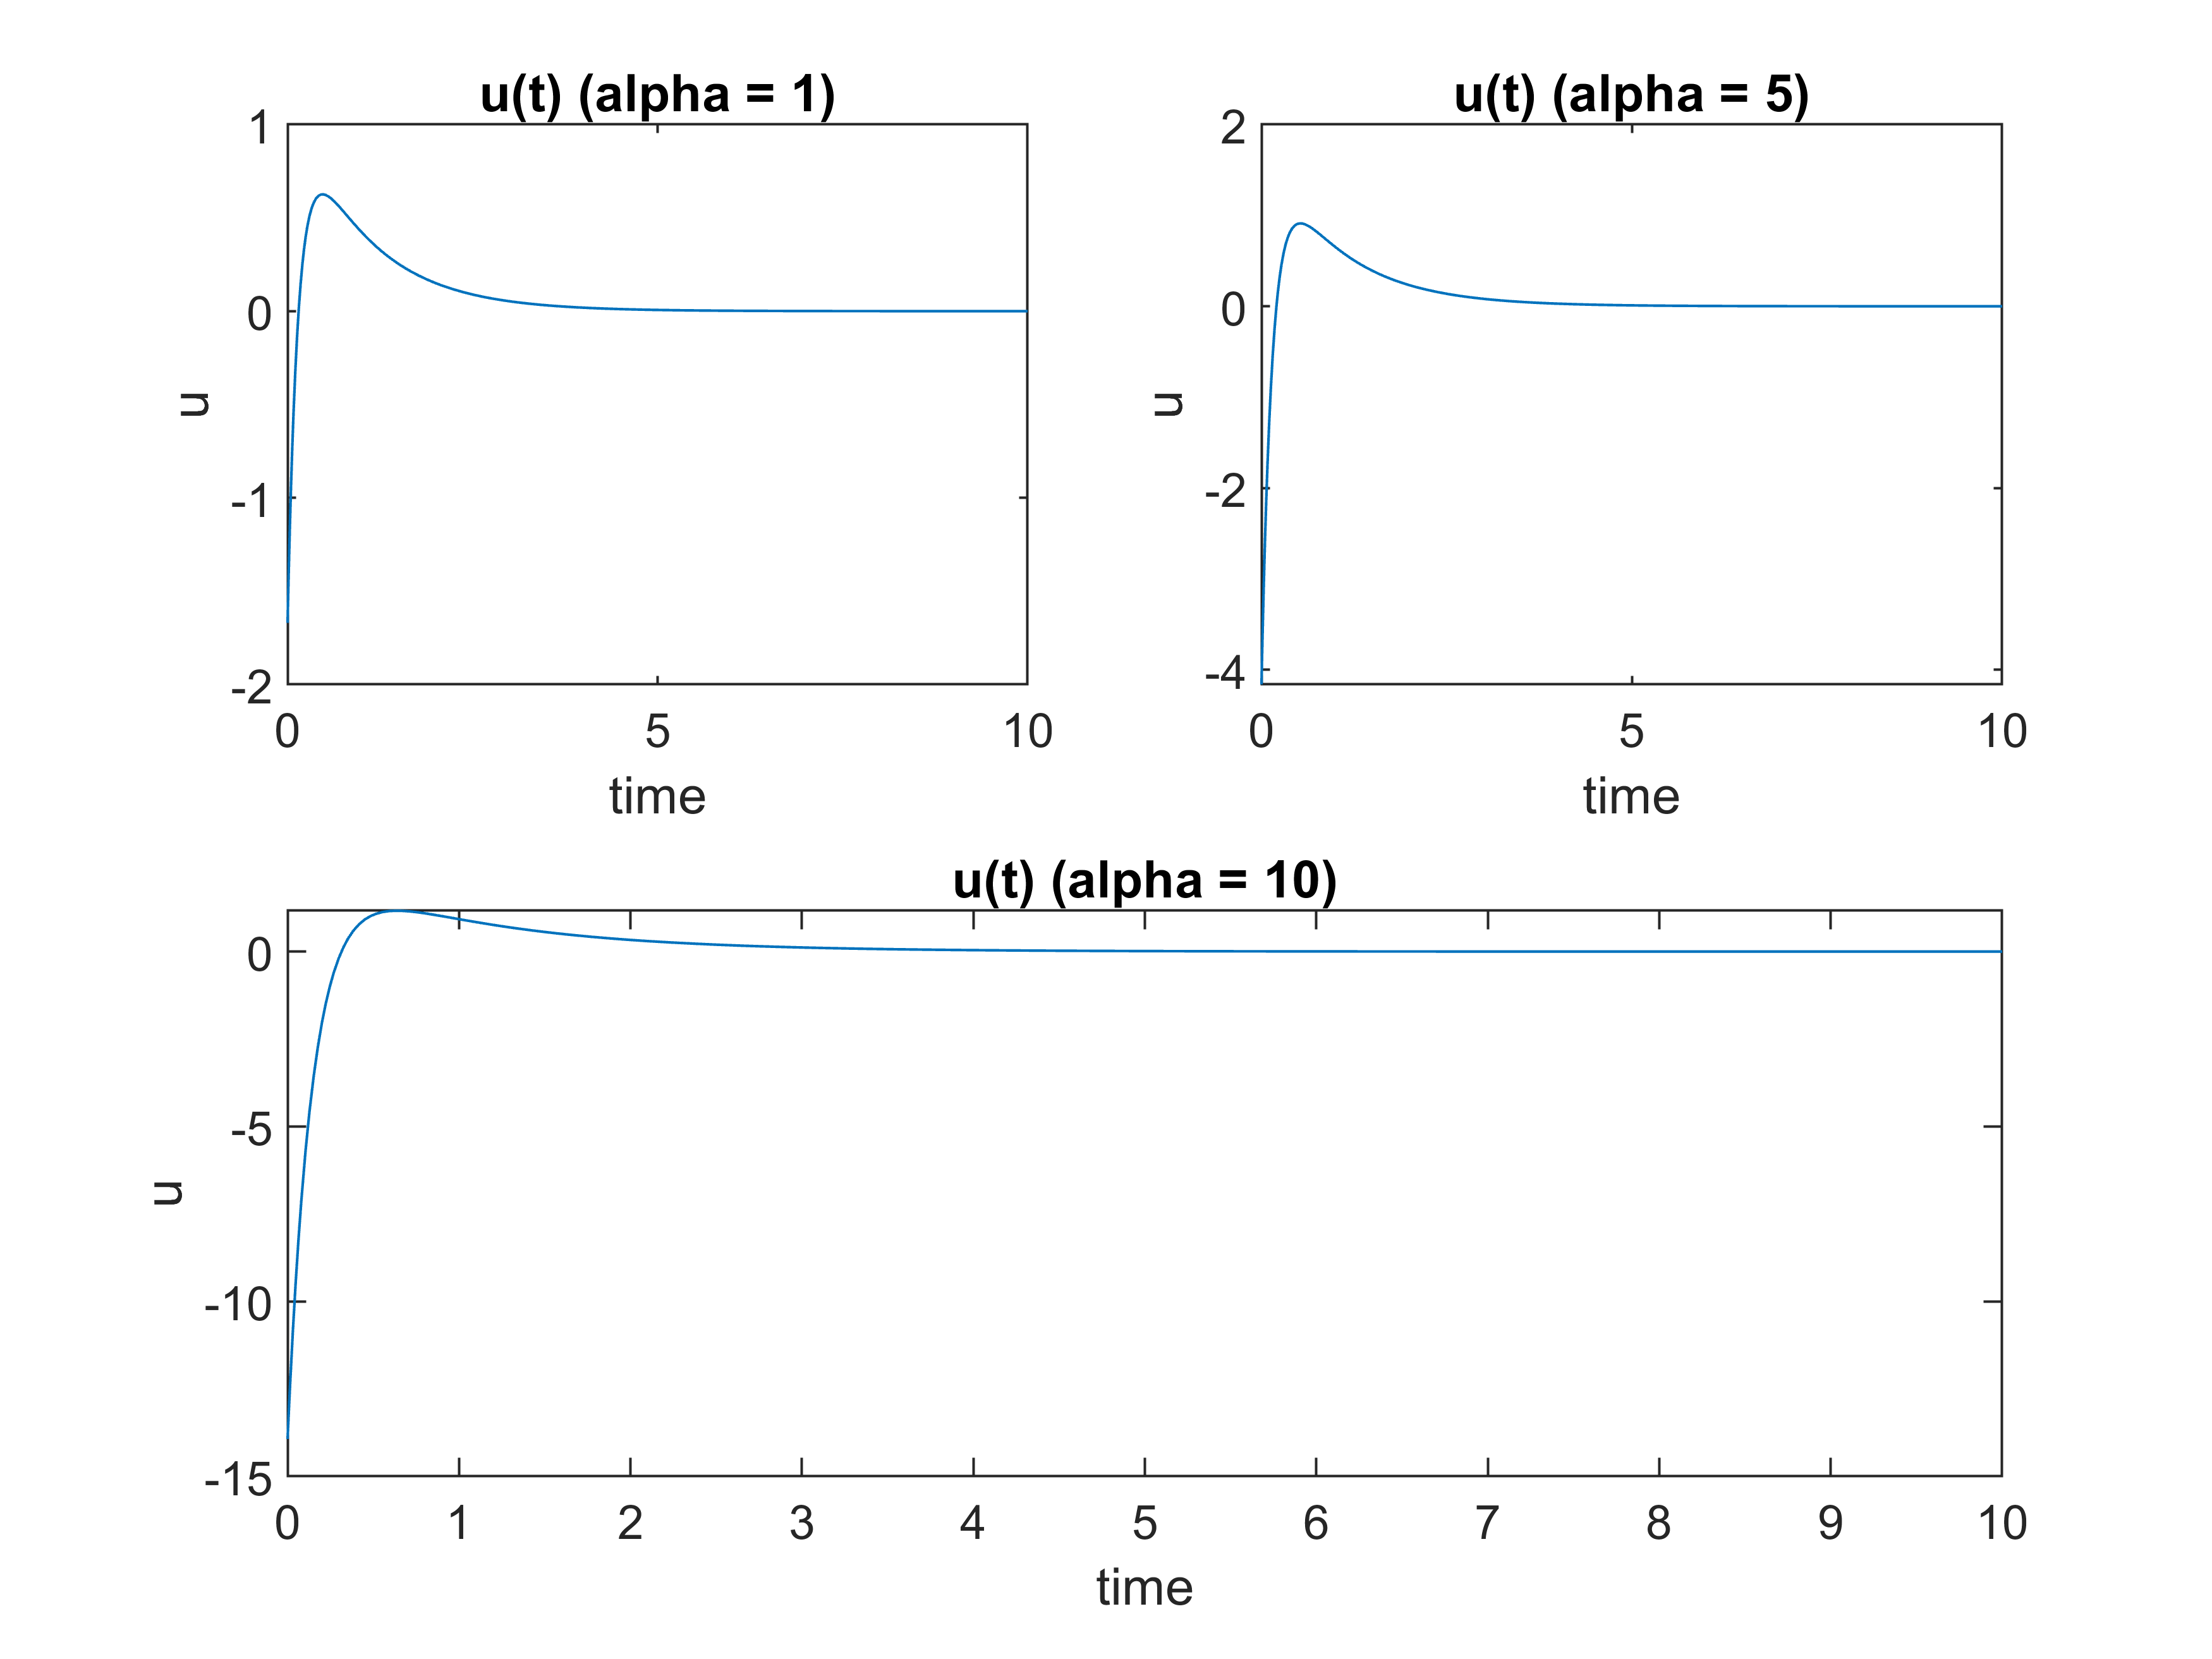
\includegraphics[width=12cm]{../Code/Q3/figures/SubplotQ3_du.png}
\end{figure}
%%%%%%%%% x(t) sub plot %%%%%%%%%
\item System States $\vec x(t)$ for all simulated $\alpha$
\begin{figure}[H]
	\caption{System States $\vec x(t)$ for all simulated $\alpha$}
	\centering
	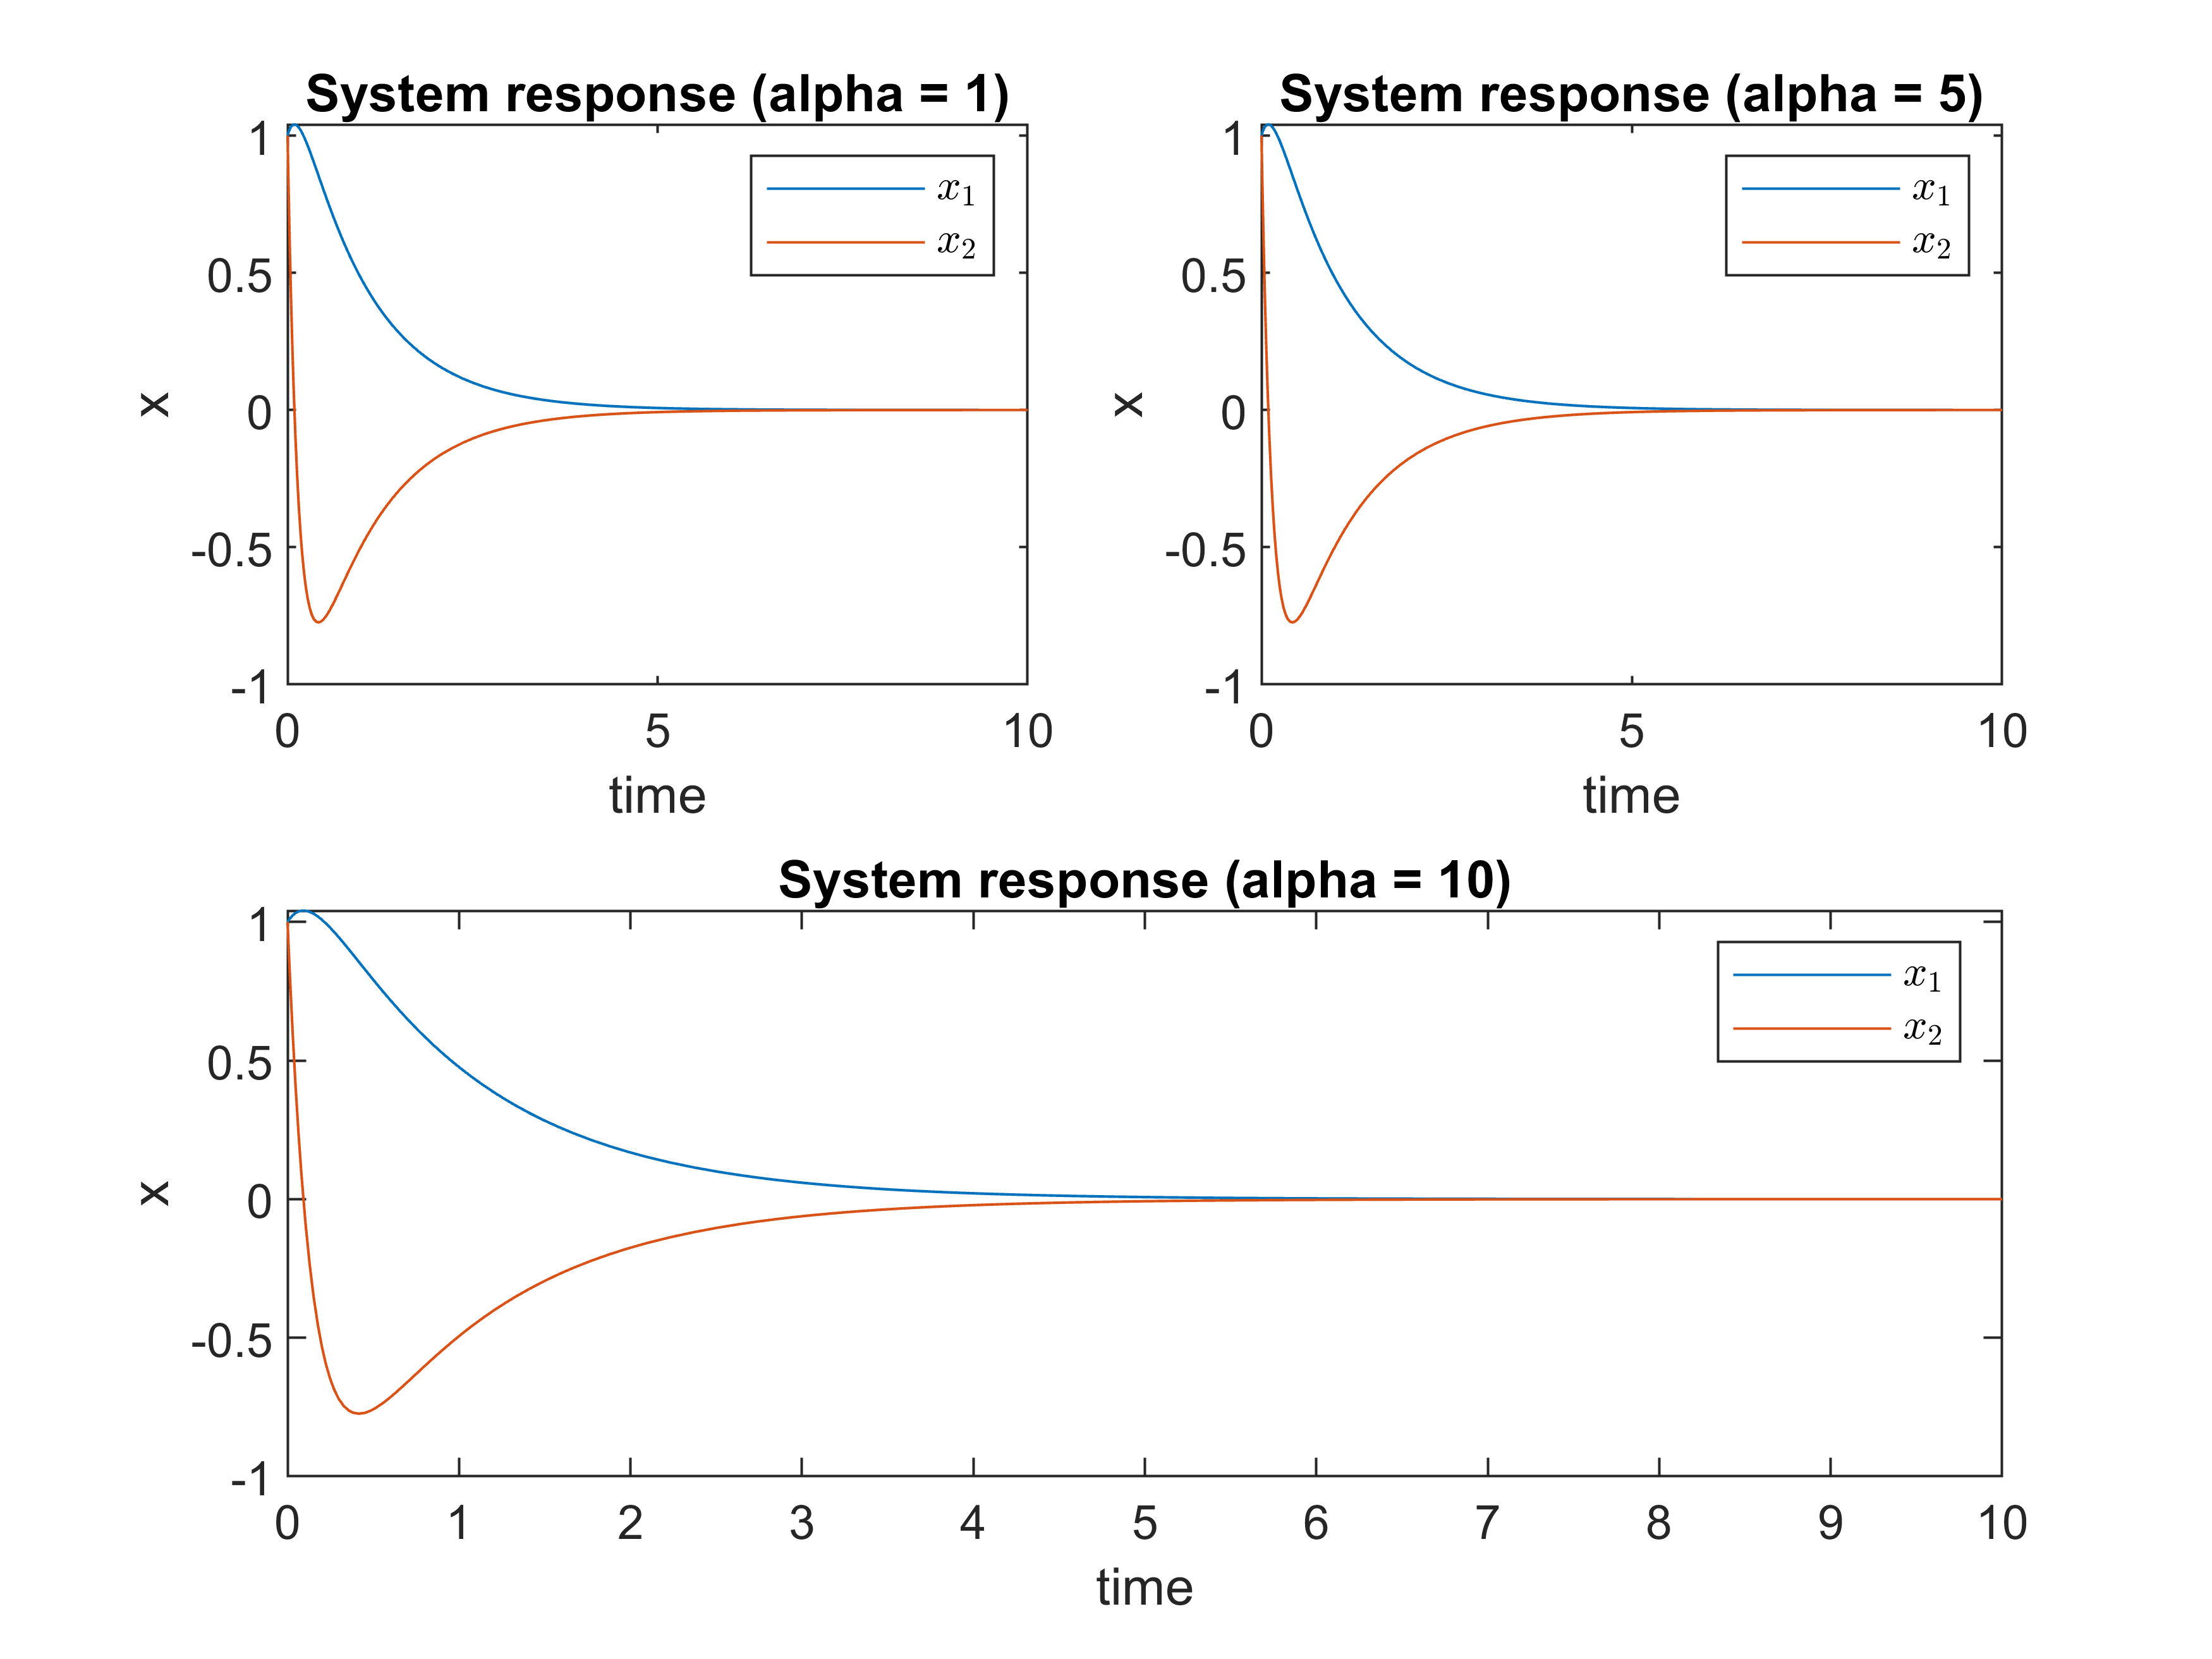
\includegraphics[width=12cm]{../Code/Q3/figures/SubplotQ3_d.png}
\end{figure}
\end{itemize}
When we increase $\alpha$ we increase position and velocity($x_1, x_2$) cost then controller use more power to go to target faster but it also use more control effort.  